\documentclass[10pt,a4paper,twocolumn,twoside]{article}
\usepackage[utf8]{inputenc}
\usepackage[T1]{fontenc}
\usepackage[catalan]{babel}
\usepackage{multicol}
\usepackage{graphicx}
\usepackage{fancyhdr}
\usepackage{times}
\usepackage{titlesec}
\usepackage{multirow}
\usepackage{lettrine}
\usepackage[top=2cm, bottom=1.5cm, left=2cm, right=2cm]{geometry}
\usepackage[figurename=Fig.,tablename=TAULA]{caption}
\captionsetup[table]{textfont=sc}

% Additional packages needed by content
\usepackage{amsmath}
\usepackage{amssymb}
\usepackage{booktabs}
\usepackage{csvsimple}
\usepackage{subcaption}
\usepackage{longtable}
\usepackage{array}
\usepackage[hypertexnames=false]{hyperref}
\usepackage{float}

\author{\LARGE\sffamily Arnau Garriga Torné}
\title{\LARGE{\sffamily Disseny i avaluació d'una metodologia d'industrialització de la Root Cause Analysis (RCA) basada en models de Machine Learning}}
\date{}

\newcommand\blfootnote[1]{%
  \begingroup
  \renewcommand\thefootnote{}\footnote{#1}%
  \addtocounter{footnote}{-1}%
  \endgroup
}

\titleformat{\section}
{\large\sffamily\scshape\bfseries}
{\textbf{\thesection}}{1em}{}

\begin{document}

\fancyhead[LO]{\scriptsize AUTOR: Arnau Garriga Torné. TÍTOL: Disseny i avaluació d'una metodologia d'industrialització de la RCA basada en ML}
\fancyhead[RO]{\thepage} \fancyhead[LE]{\thepage}
\fancyhead[RE]{\scriptsize EE/UAB TFG DADES: Industrialització RCA amb ML}

\fancyfoot[CO,CE]{}

\fancypagestyle{primerapagina}
{
   \fancyhf{}
   \fancyhead[L]{\scriptsize TFG EN ENGINYERIA DADES, ESCOLA D'ENGINYERIA (EE), UNIVERSITAT AUTÒNOMA DE BARCELONA (UAB)}
   \fancyfoot[C]{\scriptsize Juny de 2026, Escola d'Enginyeria (UAB)}
}

\renewcommand{\headrulewidth}{0pt}
\renewcommand{\footrulewidth}{0pt}
\pagestyle{fancy}

\twocolumn[\begin{@twocolumnfalse}

\maketitle

\thispagestyle{primerapagina}

\begin{center}
\parbox{0.915\textwidth}
{\sffamily
\textbf{Resum--}
Aquest treball proposa i valida una metodologia d'industrialització de la Root Cause Analysis (RCA) basada en models de Machine Learning interpretables per a entorns farmacèutics regulats. La proposta s'estructura en cinc capes: anàlisi exploratòria, modelització predictiva, estratègia \emph{filter-then-interact} amb Explainable Boosting Machines (EBM), capa d'explicabilitat i capa de validació i industrialització. El conjunt de dades utilitzat per a la modelització inclou 956 mostres i 56 variables originals, amb validació creuada de 5 folds i criteris de robustesa orientats a ús operatiu. Els resultats mostren una millora progressiva respecte al baseline Lasso: reducció del 15.6\% en MAE i del 16.9\% en RMSE en la millor configuració de Fase 4. La configuració Robust (Leaf=10) obté el millor equilibri global (MAE = 0.950, RMSE = 1.368, R² = 0.422), mantenint estabilitat entre folds i facilitant la priorització de factors crítics en RCA. Com a contribució principal, el treball demostra que una estratègia EBM interpretable-by-design permet combinar rendiment predictiu, traçabilitat i utilitat operativa, i constitueix una base sòlida per a desplegament progressiu en entorns GMP/QMS amb monitoratge de \emph{drift} i governança de cicle de vida del model.
\\
\\
\textbf{Paraules clau-- } Root Cause Analysis, Explainable Boosting Machine, interpretabilitat, validació creuada, industrialització, qualitat farmacèutica.\\
\\
\bigskip
\\
\textbf{Abstract--} This work proposes and validates an industrialisation methodology for Root Cause Analysis (RCA) based on interpretable Machine Learning models for regulated pharmaceutical environments. The proposal is structured in five layers: exploratory analysis, predictive modelling, a \emph{filter-then-interact} strategy with Explainable Boosting Machines (EBM), an explainability layer and a validation and industrialisation layer. The dataset used for modelling includes 956 samples and 56 original variables, with 5-fold cross-validation and robustness criteria oriented to operational use. Results show progressive improvement over the Lasso baseline: 15.6\% reduction in MAE and 16.9\% in RMSE in the best Phase 4 configuration. The Robust (Leaf=10) configuration achieves the best overall balance (MAE = 0.950, RMSE = 1.368, R² = 0.422), maintaining stability across folds and facilitating the prioritisation of critical factors in RCA. As a main contribution, the work demonstrates that an interpretable-by-design EBM strategy can combine predictive performance, traceability and operational utility, constituting a solid foundation for progressive deployment in GMP/QMS environments with drift monitoring and model lifecycle governance.
\\
\\
\textbf{Keywords-- } Root Cause Analysis, Explainable Boosting Machine, interpretability, cross-validation, industrialisation, pharmaceutical quality.\\
}

\bigskip

{\vrule depth 0pt height 0.5pt width 4cm\hspace{7.5pt}%
\raisebox{-3.5pt}{\fontfamily{pzd}\fontencoding{U}\fontseries{m}\fontshape{n}\fontsize{11}{12}\selectfont\char70}%
\hspace{7.5pt}\vrule depth 0pt height 0.5pt width 4cm\relax}

\end{center}

\bigskip

\end{@twocolumnfalse}]

\blfootnote{$\bullet$ E-mail de contacte: arnaugarrigatorne@gmail.com}
\blfootnote{$\bullet$ Treball tutoritzat per: Joan Piedrafita (Enginyeria de dades)}
\blfootnote{$\bullet$ Curs 2025/26}

\section{Introducció i Objectius}

La indústria farmacèutica opera sota requisits estrictes de qualitat i traçabilitat. Quan es detecta una desviació de procés o resultat fora d'especificació, cal activar una investigació de causes arrel (RCA) per identificar l'origen del problema i definir accions correctives. Malgrat la maduresa normativa del sector, aquestes investigacions continuen sent manuals i dependents de l'experiència, generant variabilitat entre investigadors, escalabilitat limitada i dificultat per garantir consistència temporal.

En aquest treball, el problema s'analitza en el context del fraccionament de plasma humà fins a l'obtenció de la Fracció II+III. Aquest procés reuneix les condicions que fan un cas d'ús especialment idoni per a ML: alta dimensionalitat (més de 150 variables de procés), variabilitat inherent de la matèria primera biològica, interaccions no lineals entre paràmetres fisicoquímics i un volum de dades històriques suficient per entrenar models robustos. A més, la seva estructura multietapa i la sensibilitat del \emph{yield} a petites desviacions operatives el converteixen en un banc de proves representatiu de processos farmacèutics complexos, de manera que la metodologia desenvolupada és transferible a altres línies de producció amb característiques similars (biotecnologia, API químics, productes estèrils). Es tracta, per tant, d'un procés farmacèutic multietapa especialment sensible a variacions fisicoquímiques i operatives. Aquesta complexitat fa que petites desviacions de procés puguin traduir-se en impactes rellevants sobre el \emph{yield} i els atributs crítics de qualitat, reforçant l'interès d'una aproximació RCA assistida per dades \cite{cohn1946,burnouf2007_modern}.

L'aparició de tècniques de Machine Learning i mètodes d'explicabilitat (XAI) permet una RCA més sistemàtica i basada en dades \cite{shap_arxiv1705,lime_arxiv1602,doshi2017rigorous}. Aquest treball proposa una metodologia d'\textbf{industrialització de la RCA basada en ML interpretable} per augmentar el criteri expert amb evidència quantitativa prioritzada, reduint l'espai d'hipòtesis i millorant la velocitat d'investigació. La proposta integra preparació de dades, modelització amb Explainable Boosting Machines (EBM), explicabilitat nativa i validació orientada a entorns regulats GxP.

\textbf{Objectius:} (1) Definir un marc RCA data-driven alineat amb requisits GxP; (2) Construir un pipeline de dades reproduïble; (3) Desenvolupar models ML interpretables per predir desviacions; (4) Aplicar tècniques d'explicabilitat per prioritzar hipòtesis de causa arrel; (5) Proposar una arquitectura d'industrialització i validació per a integració progressiva en operació.

\section{Estat de l'art}

\subsection{RCA tradicional i limitacions en entorns data-rich}

Les metodologies clàssiques de RCA (5 Whys, Ishikawa, FMEA) han estat àmpliament utilitzades en la indústria farmacèutica per estructurar investigacions de desviació. Tanmateix, diversos treballs evidencien limitacions quan el volum i heterogeneïtat de dades augmenten: dependència elevada del coneixement tàcit, baixa repetibilitat entre equips i dificultat per capturar interaccions multivariants complexes.

En entorns GxP, l'RCA requereix evidència auditable i justificació de decisions. Per això, l'objectiu no és automatitzar la decisió final, sinó reforçar la capacitat d'anàlisi de l'equip investigador amb eines quantitatives que prioritzin hipòtesis de manera transparent.

\subsection{Machine Learning i explicabilitat per a qualitat de processos}

En els darrers anys, l'aplicació de ML en qualitat farmacèutica ha crescut en casos com detecció d'anomalies, manteniment predictiu i predicció de lots fora d'especificació, utilitzant models com \emph{random forest}, \emph{gradient boosting} \cite{xgboost} o xarxes neuronals. Tanmateix, en escenaris RCA regulats, una bona mètrica predictiva és condició necessària però no suficient: cal demostrar robustesa, estabilitat temporal i, especialment, interpretabilitat operativa \cite{doshi2017rigorous,rudin2021fundamental}.

Les tècniques XAI (SHAP \cite{shap_arxiv1705}, LIME \cite{lime_arxiv1602}) han permès avançar en la transformació de prediccions en hipòtesis investigables, actuant com a mecanisme de \textbf{priorització d'hipòtesis} per reduir l'espai de recerca. Diversos treballs destaquen la diferència entre models orientats al rendiment i models interpretable-by-design que, amb compromís moderat en exactitud, faciliten la justificació de resultats i adopció en processos de qualitat.

\subsection{Explainable Boosting Machines: estat actual}

Els \emph{Explainable Boosting Machines} (EBM) representen una extensió moderna dels \emph{Generalized Additive Models} (GAMs) \cite{hastie1990_gam} que combina interpretabilitat nativa amb capacitat predictiva competitiva. Els treballs de Lou et al. \cite{lou2013_ga2m} i Caruana et al. \cite{caruana2015_intelligible} van establir les bases dels models GA2M (GAMs amb interaccions de parell), demostrant que és possible capturar interaccions controlades mantenint una estructura additiva llegible.

La literatura recent mostra que els EBM assoleixen rendiment comparable a \emph{Random Forest} o \emph{Boosted Trees}, amb l'avantatge d'un funcionament intern directament explicable \cite{ebm_nori,piml_ebm,ebm_2025}. A diferència dels models \emph{black box}, l'EBM pertany a la família \emph{glass box} i permet descriure explícitament la contribució de cada variable i interacció a la predicció, facilitant la comunicació amb experts de domini i la seva adopció en contextos on la transparència és crítica.

\subsection{Industrialització i validació en entorns GxP}

La literatura de regulació digital i validació de sistemes computaritzats (GAMP 5 \cite{gamp5}, ALCOA+ \cite{alcoa}) estableix la necessitat de definir l'ús previst, control de canvis, traçabilitat de dades/models i monitoratge continu del rendiment per garantir que una solució ML sigui defensable en auditoria. Diversos treballs destaquen també el risc de \emph{drift} \cite{lu2020drift} i la necessitat de governança del cicle de vida del model.

Com a síntesi, l'estat de l'art mostra que existeixen peces madures (RCA estructurat, modelització predictiva, XAI, qualitat de dades), però manca sovint una metodologia integral que les uneixi de forma operativa i compatible amb entorns regulats. Aquesta és precisament la bretxa que aborda el present treball: utilitzar un model interpretable-by-design com l'EBM per prioritzar hipòtesis de causa arrel amb criteris tècnics, traçables i alineats amb requisits GxP.
\section{Dades}

\subsection{Context del dataset}

El conjunt de dades integra informació de producció, control de qualitat, sensors de procés i metadades operatives d'un procés de fraccionament de plasma humà. Es disposa de \textbf{4.600 lots} al llarg de \textbf{9 anys}, amb \textbf{150 paràmetres} agrupats en blocs funcionals: variables de procés (temperatura, pressió, temps), qualitat (potència, impureses), context operatiu (torn, operador, equip), manteniment i marques temporals.

El cas d'estudi tracta del procés industrial de fraccionament de plasma humà, que té com a objectiu separar proteïnes terapèutiques de gran valor. Aquest procés es basa en el mètode de fraccionament amb etanol en fred desenvolupat per Cohn, que utilitza canvis controlats de pH, temperatura i concentració d'etanol per separar diferents proteïnes \cite{cohn1946,burnouf2007_modern}. Tot i que actualment el procés inclou etapes avançades de purificació, el rendiment i la seguretat del producte depenen principalment de les primeres etapes de separació \cite{burnouf2007_modern}.

Aquest treball se centra en la producció fins a l'obtenció de la Fracció II+III, on es concentra la major part de les immunoglobulines (IgG). El tram analitzat inclou tres fases clau: (1) separació inicial, que inclou la descongelació del plasma i la recuperació del crioprecipitat, amb el temps de barreja (\emph{pooling}) i l'edat del plasma com a factors més rellevants; (2) precipitació de proteïnes, on se separen les Fraccions I i II+III mitjançant l'addició d'etanol i l'ajust del pH, etapa en què són crítics la precisió en l'addició d'etanol, el control del pH i el temps de mescla; i (3) filtració i recuperació, que es realitza amb filtres premsa i papers de diferent gruix, i determina el rendiment final (\emph{yield}) i la claredat del filtrat \cite{burnouf2007_modern,cohn1946}.

El procés és altament variable perquè el plasma és una matèria primera biològica i les proteïnes són especialment sensibles als canvis de temperatura i a les condicions químiques \cite{burnouf2007_modern,gamp5}. En aquest context, petites variacions en paràmetres operatius com la pressió de les centrífugues, la quantitat de tampó afegit o el temps de filtració poden afectar directament la recuperació de la IgG i la qualitat del producte final. Per aquest motiu, és necessari utilitzar eines avançades d'anàlisi de causes arrel (RCA), que permetin reduir la variabilitat del procés i prioritzar les investigacions, assegurant el compliment de la normativa GxP.

A partir del \textbf{2024} s'observa un canvi de procés que coincideix amb una millora del \emph{yield}. Atesa la no-estacionarietat del procés, l'entrenament es focalitza en dades \textbf{des de 2024} (\textbf{960 lots}) per garantir homogeneïtat operacional. Del total de 150 variables, \textbf{104 són numèriques} i \textbf{46 categòriques}.

\subsection{Qualitat de dades, neteja i preparació}

La neteja no s'ha fet de manera mecànica, sinó amb criteri de domini i validació experta, alineant-se amb la literatura sobre interpretabilitat i selecció de variables en contextos industrials \cite{nori2019_unified,guyon2003_feature_selection,liu2021_missing_industrial,boloncanedo2015_review}. S'han analitzat valors absents per variable i causa operacional, correlacions fortes per evitar redundàncies i multicol·linearitat, variables de variància baixa amb aportació limitada, i variables temporals amb baixa utilitat causal directa.

S'ha construït un mapa de variables per documentar descripció funcional, fase del procés, naturalesa accionable i relacions entre variables. Cada variable inclou atributs com descripció, fase, accionabilitat i correlacions, facilitant la separació de variables operatives, informatives i descriptives.

També s'han aplicat transformacions de \emph{feature engineering}, substituint marques temporals puntuals per durades agregades més robustes (p.~ex. temps total de fase), reduint soroll i concentrant el model en factors rellevants del comportament de procés.

\subsection{Partició temporal i govern de dades}

La partició de dades es realitza cronològicament dins del període 2024+ per evitar fuites d'informació. El dataset final conté \textbf{956 mostres i 56 variables}. Per garantir traçabilitat \emph{end-to-end}, s'ha establert versionat de datasets, diccionari de dades i registre de transformacions.

% ======================================================================
% METODOLOGIA - Enhanced LaTeX with Figures and Tables (Version 2)
% ======================================================================
% Required packages:
% \usepackage{graphicx}
% \usepackage{booktabs}
% \usepackage{csvsimple}
% \usepackage{caption}
% \usepackage{subcaption}

\section{Metodologia}
\label{sec:metodologia}

Aquest treball proposa una metodologia estructurada en cinc capes: anàlisi exploratòria, modelització ML (Lasso, Gradient Boosting, EBM), estratègia \emph{filter-then-interact} amb EBM en tres fases, explicabilitat per a RCA, i validació/industrialització. L'arquitectura garanteix rendiment predictiu i interpretabilitat alineada amb el domini farmacèutic.

\subsection{Capa d'anàlisi exploratòria}
\label{subsec:capa_analisi_exploratoria}

Activitats d'exploració i comprensió del conjunt de dades:

\begin{enumerate}
    \item \textbf{Anàlisi de la distribució de variables:} Estudi de la distribució de la variable objectiu (qualitat de la proteïna) i de les variables predictores.
    \item \textbf{Detecció de valors atípics:} Identificació de dades anòmales que poden afectar el rendiment dels models.
    \item \textbf{Anàlisi de correlacions:} Estudi de les relacions lineals entre variables per detectar redundàncies i possibles col·linealitats.
    \item \textbf{Reducció de dimensionalitat basada en correlació:} Eliminació de variables altament correlacionades per simplificar el model i evitar multicolinealitat.
    \item \textbf{Anàlisi de qualitat de les dades:} Avaluació de la completesa i consistència de les dades, així com la identificació de valors faltants.
\end{enumerate}

\subsection{Capa de modelització de ML}
\label{subsec:capa_modelitzacio_ml}

Es van avaluar tres famílies de models per establir una línia base:

\begin{enumerate}
    \item \textbf{Lasso (Least Absolute Shrinkage and Selection Operator):} Model lineal amb regularització L1 que realitza selecció de característiques de manera automàtica. Aquest model serveix com a línia base i proporciona una primera aproximació a les variables més rellevants.

    \item \textbf{Gradient Boosting (XGBoost/LightGBM):} Models d'ensemble basats en arbres de decisió que capturen relacions no lineals complexes. Aquests models ofereixen alt rendiment predictiu però són menys interpretables.

    \item \textbf{Explainable Boosting Machine (EBM):} Model additiu generalitzat (GAM) basat en boosting que manté la interpretabilitat mentre captura efectes no lineals i interaccions entre variables.
\end{enumerate}

\subsubsection{Model de línia base: Lasso}
\label{subsubsec:model_baseline_lasso}

El model Lasso va aconseguir MAE = 1.126, RMSE = 1.646 i R² = 0.332 sobre el conjunt de test.

Les variables més rellevants identificades pel Lasso inclouen pes de fraccions específiques (D23, C29) i paràmetres de filtració (D36, D24), establint la base per a l'estratègia amb EBM.

\subsection{Estratègia filter-then-interact amb EBM}
\label{subsec:estrategia_filter_then_interact}

L'estratègia \emph{filter-then-interact} captura efectes principals i interaccions en tres fases progressives, minimitzant overfitting i maximitzant interpretabilitat. Aquesta aproximació s'alinea amb la metodologia proposada per Lou et al.~\cite{lou2013_ga2m} per als models GA$^2$M, on s'aïllen primer els efectes principals per garantir l'estabilitat de les shape functions i, posteriorment, s'activen les interaccions de parella més significatives de manera controlada, tal com van demostrar Caruana et al.~\cite{caruana2015_intelligible} en entorns on la transparència regulatòria és crítica.

\subsubsection{Fase 1: Identificació d'efectes principals}
\label{subsubsec:fase1_efectes_principals}

S'entrena un model EBM sense interaccions (\texttt{interactions=0}) per capturar únicament els efectes principals de cada variable.

Hiperparàmetres: \texttt{interactions=0}, \texttt{learning\_rate=0.05}, \texttt{max\_bins=256}, \texttt{max\_rounds=5000}, \texttt{min\_samples\_leaf=2}.

El model EBM va aconseguir MAE = 1.072, RMSE = 1.602 i R² = 0.368, superant el baseline Lasso i capturant relacions no lineals.

\begin{figure}[htbp]
    \centering
    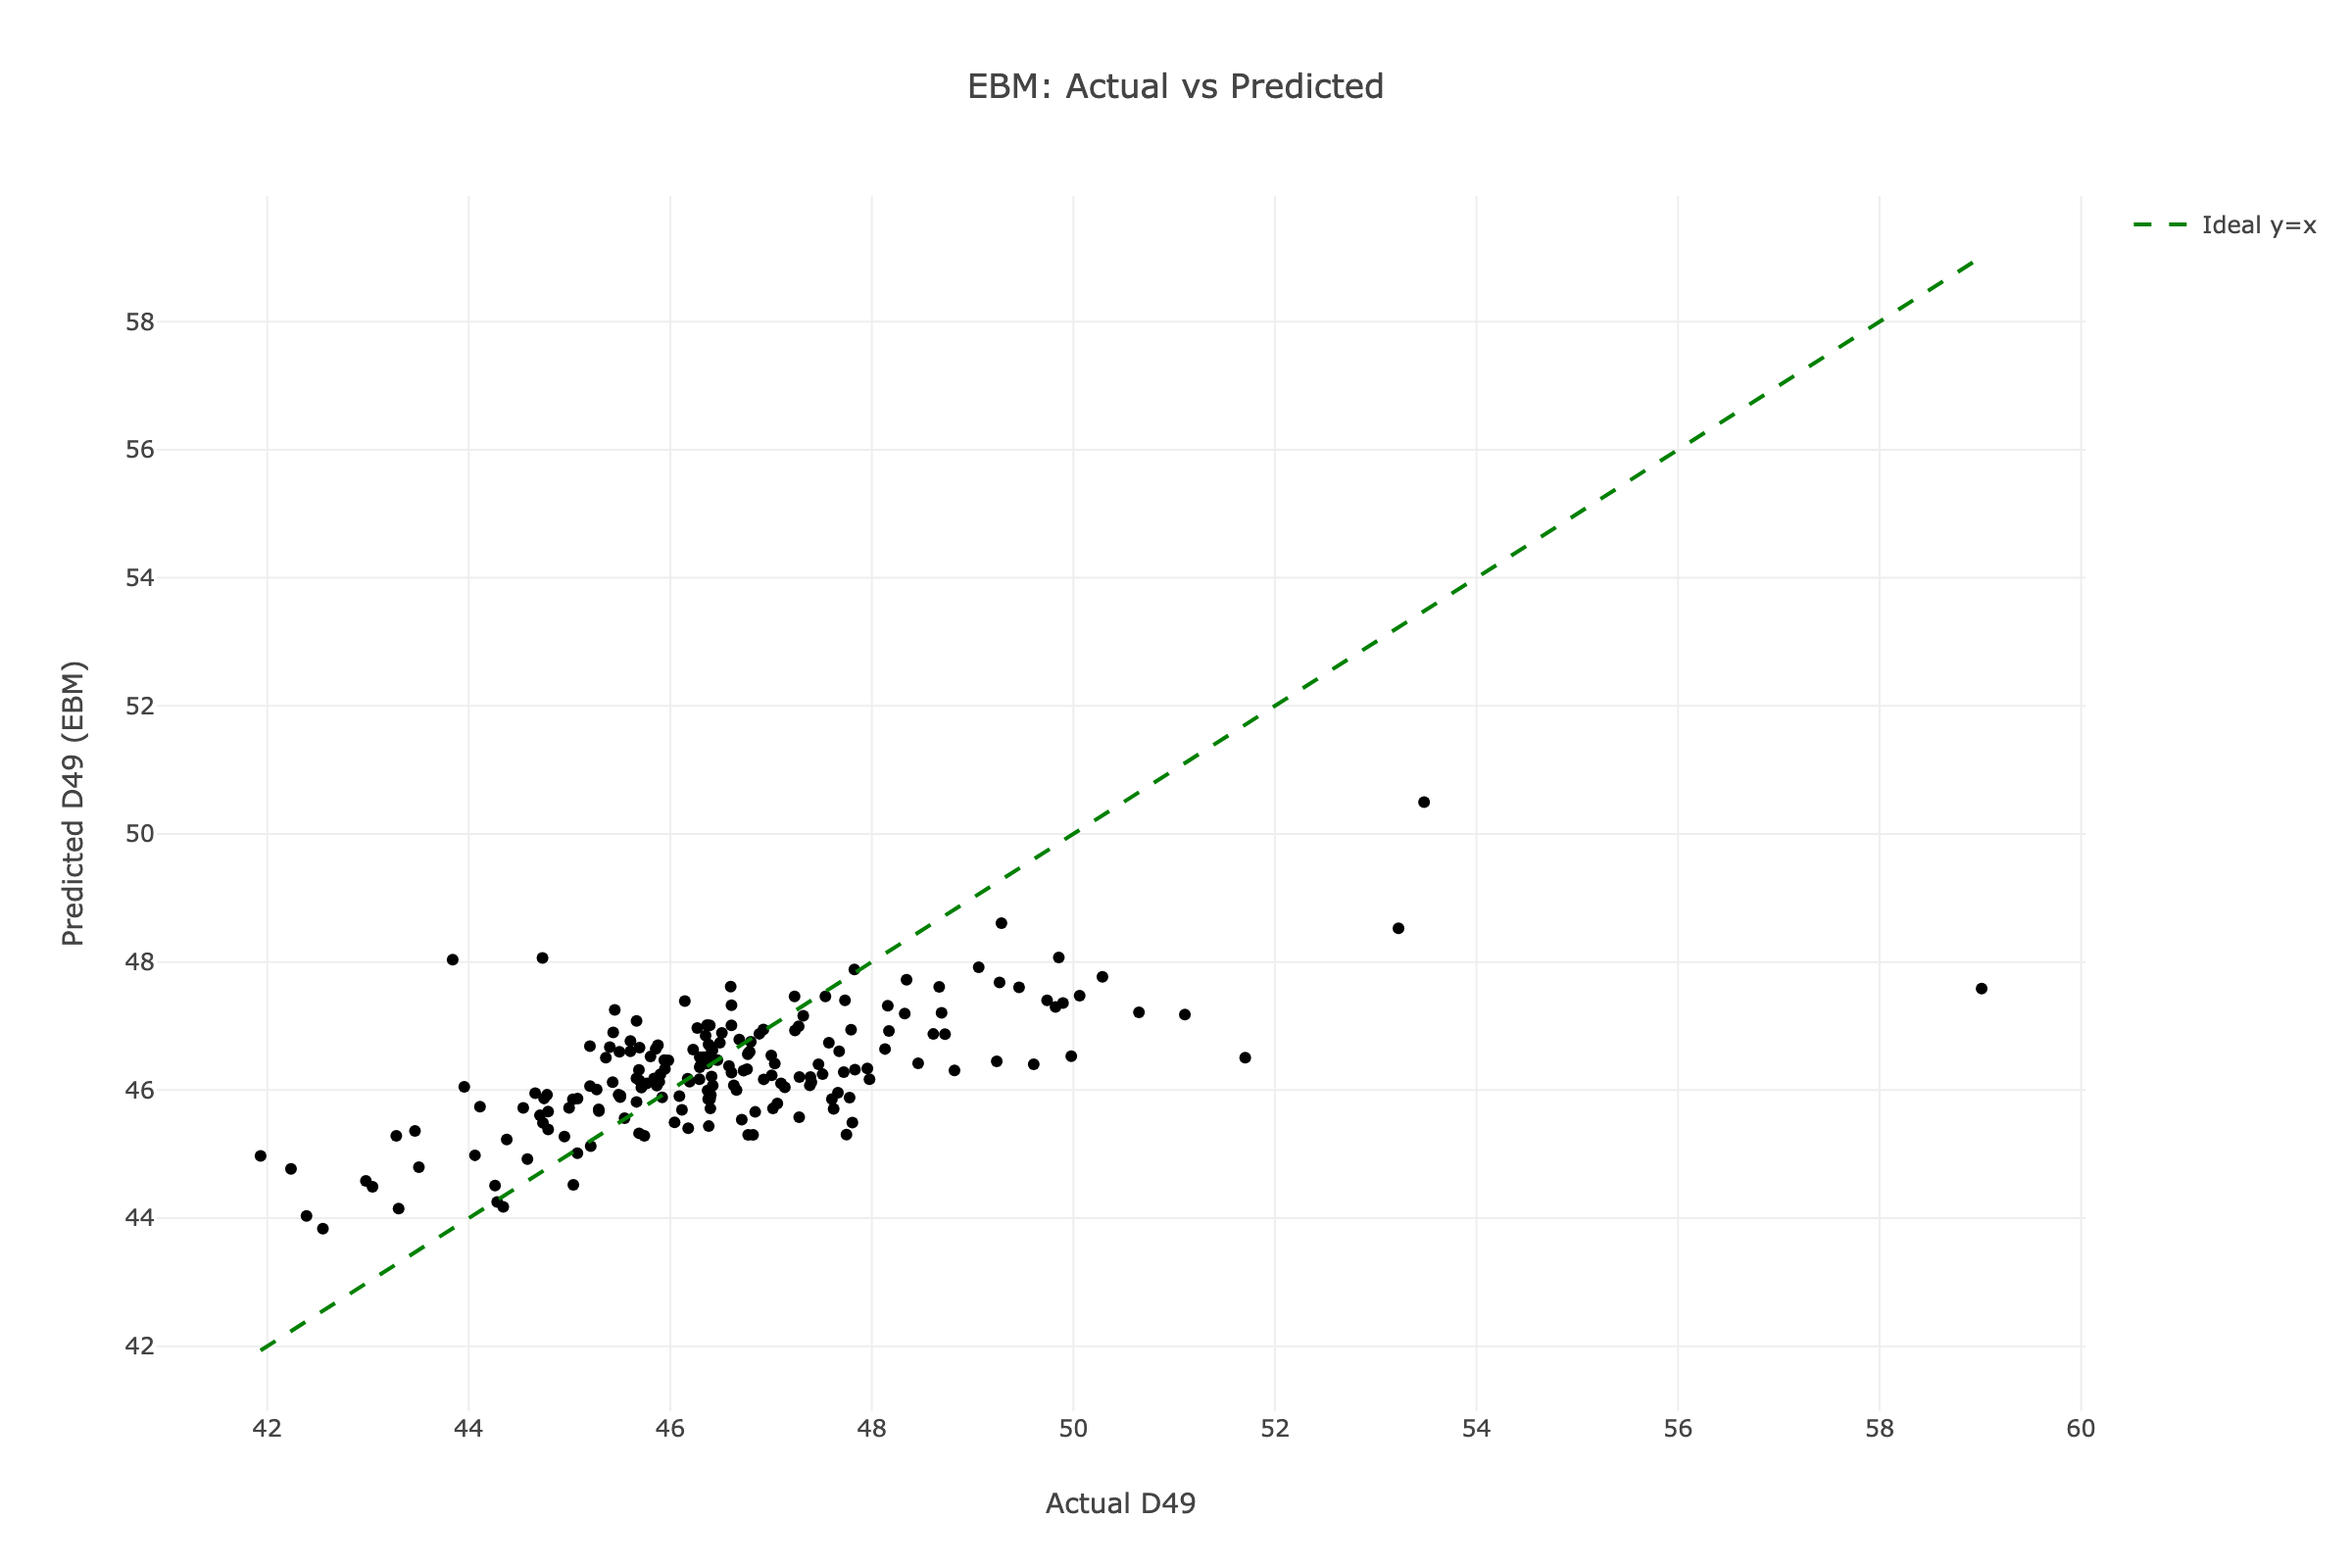
\includegraphics[width=\columnwidth]{images/fig_008_match_lasso_behavior_show_human_readable_name_next_to_encoded_feature_key.png}
    \caption{Predicció vs valor real (D49) del model EBM Fase 1 (sense interaccions). La línia discontínua representa la predicció perfecta ($y=x$).}
    \label{fig:ebm_phase1_actual_vs_pred}
\end{figure}

\subsubsection{Fase 2: Filtrat i reducció de dimensionalitat}
\label{subsubsec:fase2_filtrat_dimensionalitat}

Selecció de característiques basada en la importància apresa en Fase 1, reduint dimensionalitat i facilitant captura d'interaccions significatives.

\paragraph{Prova preliminar: Lasso $\rightarrow$ EBM (Top-10)}
Es va utilitzar el model Lasso com a filtre inicial, seleccionant les 10 característiques amb major importància per entrenar un model EBM.

El model EBM amb Top-10 Lasso va aconseguir MAE = 1.072, RMSE = 1.602, R² = 0.368.

La configuració final va seleccionar les \textbf{15 característiques més importants} (\texttt{top\_n = 15}), identificant el punt on la importància experimenta una caiguda significativa i mantenint variables amb major poder predictiu.

\subsubsection{Fase 3: Captura controlada d'interaccions}
\label{subsubsec:fase3_captura_interaccions}

La tercera i última fase entrena un model EBM sobre el conjunt reduït de característiques seleccionades en la Fase 2, activant la detecció automàtica d'interaccions. Aquesta configuració permet que el model identifiqui fins a 25 parells d'interaccions significatives (\texttt{interactions=25}) de manera automàtica.

Hiperparàmetres: \texttt{interactions=10} (detecció automàtica), \texttt{learning\_rate=0.05}, \texttt{max\_bins=256}, \texttt{max\_rounds=5000}, \texttt{min\_samples\_leaf=10}.

El model final va aconseguir un rendiment significativament millorat: MAE = 1.018, RMSE = 1.466 i R² = 0.470, demostrant l'efectivitat de la captura d'interaccions de manera controlada.

\begin{figure}[htbp]
    \centering
    \begin{subfigure}[b]{\columnwidth}
        \centering
        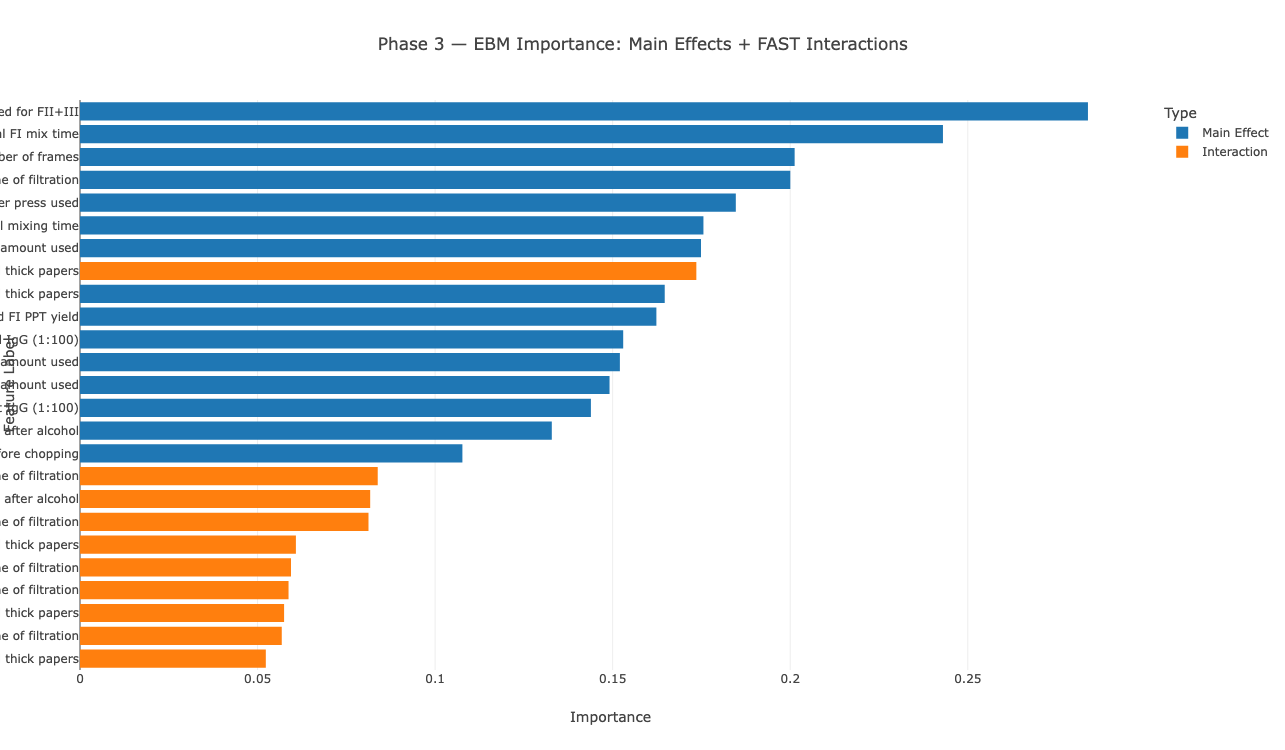
\includegraphics[width=0.95\columnwidth]{images/plot_importances.png}
        \caption{Efectes principals}
        \label{fig:ebm_phase3_main}
    \end{subfigure}
    \vspace{0.3em}
    \begin{subfigure}[b]{\columnwidth}
        \centering
        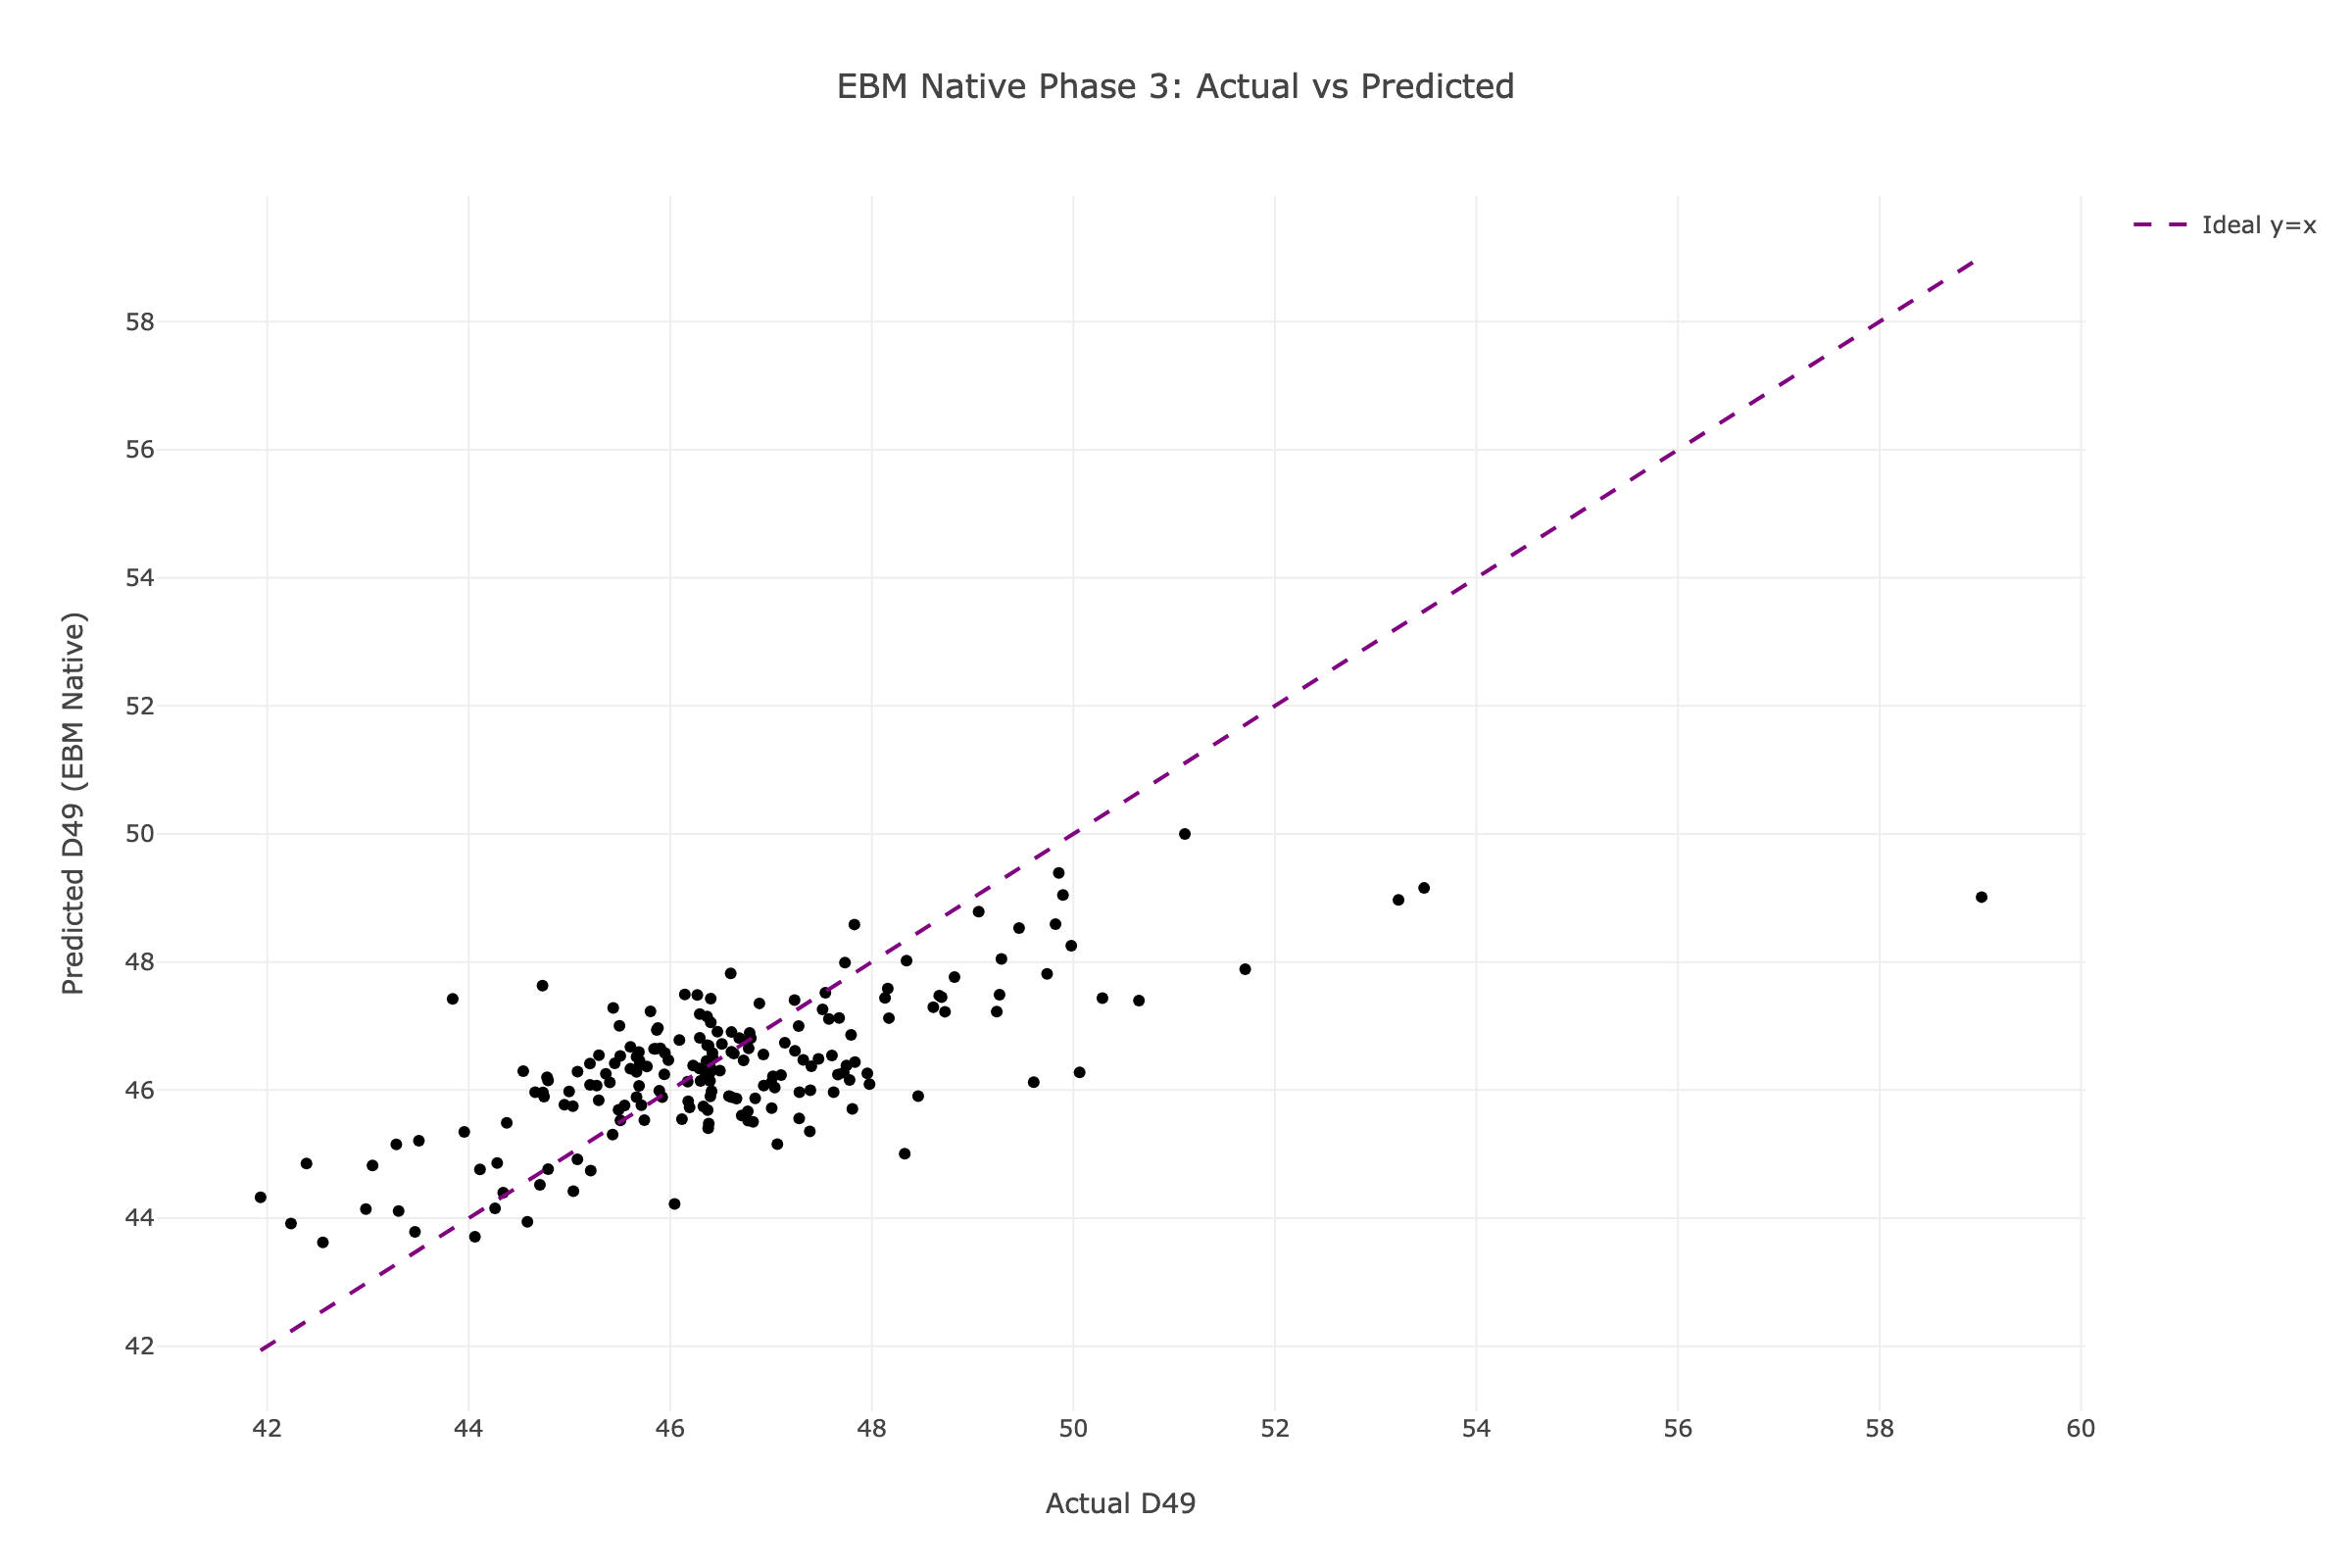
\includegraphics[width=0.95\columnwidth]{images/fig_014__extract_learned_terms_.png}
        \caption{Interaccions entre variables}
        \label{fig:ebm_phase3_interactions}
    \end{subfigure}
    \caption{Descomposició del model EBM Fase 3: (a) importància dels efectes principals de les 15 característiques seleccionades, (b) importància de les interaccions detectades automàticament pel model.}
    \label{fig:ebm_phase3_decomposition}
\end{figure}

La Figura \ref{fig:ebm_phase3_decomposition} mostra que el model captura efectes principals robustos i interaccions rellevants entre variables.

\subsubsection{Densitat de dades i control de complexitat}
\label{subsubsec:densitat_dades_control_complexitat}

La reducció de característiques (de 50+ variables a 15) redueix l'espai de cerca d'interaccions de O(n²) i garanteix suficients dades per estimar efectes principals i interaccions de manera fiable.

\subsection{Capa d'explicabilitat i Root Cause Analysis}
\label{subsec:capa_explicabilitat_rca}

Els models EBM proporcionen explicacions a diferents nivells. Tècniques utilitzades:

\begin{itemize}
    \item \textbf{Importància global de característiques:} Mesura de la contribució relativa de cada variable i interacció al rendiment general del model.
    \item \textbf{Shape functions:} Visualització de com cada característica afecta la predicció al llarg del seu rang de valors, capturant relacions no lineals.
    \item \textbf{Contribucions locals:} Descomposició de prediccions individuals per entendre quines variables i interaccions contribueixen a prediccions específiques.
    \item \textbf{Anàlisi d'interaccions:} Exploració de les relacions sinèrgiques entre parells de variables per identificar efectes combinats.
\end{itemize}

\subsection{Capa de validació i industrialització}
\label{subsec:capa_validacio_industrialitzacio}

Validació rigorosa del model i preparació per a implementació en entorns productius, garantint robustesa davant nous lots de producció.

\subsubsection{Validació d'hiperparàmetres i robustesa final}
\label{subsubsec:fase4_validacio_hiperparametres}

Es van explorar set configuracions diferents, variant bins (128, 256, 512), mostres per fulla (2, 5, 10), interaccions (15, 20, 25) i profunditat d'aprenentatge, identificant la configuració amb millor equilibri entre precisió, estabilitat i robustesa. Resultats detallats a la Secció~\ref{sec:resultats}.

\subsubsection{Preparació per a la industrialització}
\label{subsubsec:preparacio_industrialitzacio}

Aspectes clau: serialització i versionat del model (pickle/joblib amb metadades), pipeline de preprocessament documentat, sistema de monitoratge per detectar \emph{data/model drift}, integració amb sistemes MES via API REST, i documentació tècnica i operativa completa.

\subsubsection{Marc de validació GxP i posicionament del model}
\label{subsubsec:marc_validacio_gxp}

GAMP 5 \cite{gamp5} i la seva extensió per a IA/ML \cite{gamp_ai_ml} estableixen un cicle de validació basat en risc per a sistemes computaritzats en entorns GxP: especificació de requisits d'usuari (URS), avaluació de risc, qualificació d'instal·lació (IQ), operacional (OQ) i rendiment (PQ), control de canvis i monitoratge continu. La guia específica d'IA/ML \cite{gamp_ai_ml} adapta aquest cicle a models predictius, incorporant proves de rendiment estadístic, robustesa davant pertorbacions i detecció de drift com a elements d'OQ/PQ. L'Annex 11 d'EudraLex \cite{eudralex_annex11} reforça l'exigència de demostrar funcionament consistent i traçable.

El posicionament del model com a \emph{decision support} —no decisor automàtic— redueix la categoria de risc i l'esforç de validació requerit. La Taula~\ref{tab:gxp_positioning} resumeix l'estat actual respecte al marc GxP.

\begin{table}[htbp]
\centering
\caption{Posicionament del model respecte a requisits GxP}
\label{tab:gxp_positioning}
\footnotesize
\begin{tabular}{@{}p{0.42\columnwidth}p{0.50\columnwidth}@{}}
\toprule
\textbf{Cobert} & \textbf{Pendent} \\
\midrule
Interpretabilitat nativa (ALCOA+) & IQ/OQ/PQ formal \\
Pipeline documentat i versionat & Cobertura temporal ampliada \\
Monitoratge drift (PSI) & Protocol de change control \\
Ús previst delimitat (support) & Aprovació formal QA \\
Latència demostrada (OQ parcial) & Revalidació periòdica \\
\bottomrule
\end{tabular}
\end{table}

El drift detectat (PSI = 6.8 a D36) il·lustra empíricament la necessitat dels processos de revalidació que GAMP 5 exigeix. En conjunt, el treball construeix els fonaments tècnics —model interpretable, traçable i monitoritzat— sobre els quals es podria executar una validació GxP formal com a pas posterior.


% Section 6: Resultats i Discussió (fusió d'Experiments + Discussió)

\section{Resultats i Discussió}
\label{sec:resultats}

\subsection{Configuració experimental}

Tots els experiments s'han executat amb Python 3.9, InterpretML 0.4.3, scikit-learn 1.2.0, validació creuada de 5 folds (seed=42) sobre un dataset de \textbf{956 mostres i 56 variables}. Les mètriques emprades són MAE (Mean Absolute Error), RMSE (Root Mean Squared Error) i R² (Coefficient of Determination), calculades amb mitjana i desviació estàndard per avaluar estabilitat.

\subsection{Resultats quantitatius i millora progressiva}

La Taula~\ref{tab:progressive_improvement} mostra la millora progressiva des del model baseline Lasso fins a la millor configuració de Fase 4, demostrant l'efectivitat de la metodologia proposada.

\begin{table}[htbp]
\centering
\caption{Evolució progressiva del rendiment del model a través de les fases de la metodologia.}
\label{tab:progressive_improvement}
\scriptsize
\resizebox{\columnwidth}{!}{%
\begin{tabular}{@{}lrrr@{}}
\toprule
\textbf{Fase} & \textbf{MAE} & \textbf{RMSE} & \textbf{R²} \\
\midrule
Lasso (Baseline) & 1.126 & 1.646 & 0.332 \\
EBM Fase 1 & 1.072 & 1.602 & 0.368 \\
EBM Fase 3 & 1.018 & 1.466 & 0.470 \\
\textbf{EBM Fase 4 (Robust)} & \textbf{0.950} & \textbf{1.368} & \textbf{0.422} \\
\midrule
\textbf{Millora total (\%)} & \textbf{-15.6\%} & \textbf{-16.9\%} & \textbf{+27.1\%} \\
\bottomrule
\end{tabular}%
}
\end{table}

S'ha aconseguit una reducció del \textbf{15.6\% en MAE} i del \textbf{16.9\% en RMSE}, amb increment del 27.1\% en R². Cal destacar que la Fase 3 obté un R² superior (0.470) però amb menys estabilitat. La configuració \textbf{Robust (Leaf=10)} de Fase 4 ofereix el millor compromís entre precisió i robustesa: MAE = 0.950, RMSE = 1.368, R² = 0.422, amb desviacions estàndard contingudes que garanteixen estabilitat entre folds. Aquesta robustesa és crítica per a aplicació industrial, on la fiabilitat és tan important com la precisió puntual.

\subsection{Comparació de configuracions en Fase 4}

S'han avaluat set configuracions d'EBM en Fase 4, explorant diferents compromisos entre precisió, interpretabilitat i robustesa. La Taula~\ref{tab:phase4_results} mostra els resultats.

\begin{table}[htbp]
\centering
\caption{Resultats de les set configuracions d'EBM en Fase 4 amb 5-fold cross-validation.}
\label{tab:phase4_results}
\scriptsize
\resizebox{\columnwidth}{!}{%
\begin{tabular}{@{}lrrr@{}}
\toprule
\textbf{Configuració} & \textbf{MAE} $\pm$ std & \textbf{RMSE} $\pm$ std & \textbf{R²} $\pm$ std \\
\midrule
\textbf{Robust (Leaf=10)} & \textbf{0.950 $\pm$ 0.063} & \textbf{1.368 $\pm$ 0.153} & \textbf{0.422 $\pm$ 0.109} \\
High Interactions (25) & 0.953 $\pm$ 0.057 & 1.370 $\pm$ 0.136 & 0.421 $\pm$ 0.094 \\
Current Best & 0.953 $\pm$ 0.060 & 1.371 $\pm$ 0.154 & 0.420 $\pm$ 0.107 \\
High Precision (512 bins) & 0.954 $\pm$ 0.059 & 1.371 $\pm$ 0.149 & 0.420 $\pm$ 0.103 \\
Slow/Deep Learning & 0.954 $\pm$ 0.068 & 1.381 $\pm$ 0.155 & 0.412 $\pm$ 0.105 \\
Smooth Sensors (128 bins) & 0.956 $\pm$ 0.059 & 1.378 $\pm$ 0.149 & 0.415 $\pm$ 0.101 \\
Simple/Stable & 0.963 $\pm$ 0.069 & 1.411 $\pm$ 0.162 & 0.387 $\pm$ 0.108 \\
\bottomrule
\end{tabular}%
}
\end{table}

Les configuracions amb més regularització (Robust, Current Best) superen les més complexes, confirmant que amb datasets limitats (956 mostres) la simplificació del model és més beneficiosa que l'increment de capacitat representacional.

\subsection{Comparació amb models alternatius}
\label{subsec:comparacio_models_alternatius}

Un dels interrogants clau d'aquest treball és si la restricció d'interpretabilitat penalitza el rendiment predictiu. A diferència de les Taules~\ref{tab:progressive_improvement} i~\ref{tab:phase4_results}, que utilitzen validació creuada de 5 folds, els resultats d'aquesta secció corresponen al conjunt de test fix (242 mostres, 25\% del dataset) per garantir comparabilitat directa entre models amb arquitectures heterogènies. S'ha comparat el model proposat (EBM filter+interact) amb quatre alternatives representatives: (A) LASSO com a referència lineal, (B) EBM sense filtratge previ per aïllar l'efecte de la fase de \emph{pruning}, (C) XGBoost optimitzat amb GridSearchCV (48 combinacions d'hiperparàmetres) com a representant \emph{black-box}, i (D) LASSO+EBM per avaluar si la selecció lineal de variables és adequada per a models no lineals.

\begin{table}[htbp]
\centering
\caption{Benchmark comparatiu de 5 models (test set, 242 mostres).}
\label{tab:model_comparison}
\scriptsize
\resizebox{\columnwidth}{!}{%
\begin{tabular}{@{}lrrrr@{}}
\toprule
\textbf{Model} & \textbf{MAE} & \textbf{R²} & \textbf{Termes} & \textbf{Train (s)} \\
\midrule
\textbf{EBM filter+interact} & \textbf{0.994} & \textbf{0.477} & 25 & 4.9 \\
EBM full (no filter) & 1.026 & 0.395 & 66 & 11.6 \\
LASSO (full) & 1.038 & 0.383 & 36 & 0.1 \\
XGBoost tuned & 1.037 & 0.369 & 2500 & 78.2 \\
LASSO + EBM & 1.177 & 0.202 & 18 & 4.3 \\
\bottomrule
\end{tabular}%
}
\end{table}

Els resultats (Taula~\ref{tab:model_comparison} i Figura~\ref{fig:model_comparison}) demostren tres conclusions operativament rellevants:

\textbf{(1) La interpretabilitat no penalitza el rendiment.} L'EBM filter+interact supera XGBoost en R² per un marge del 29\% relatiu (0.477 vs 0.369), invalidant l'assumpció habitual que els models \emph{glass-box} sacrifiquen precisió per guanyar transparència. En el context GxP, on cada predicció ha de ser justificable davant auditoria \cite{gamp5}, aquest resultat elimina la tensió entre compliment normatiu i capacitat analítica.

\textbf{(2) El filtratge de característiques és l'element diferencial.} La comparació directa entre EBM amb i sense filtratge (R²: 0.477 vs 0.395, p=0.037 en test de Wilcoxon) demostra que reduir de 56 a 15 variables no perd informació sinó que elimina soroll que degrada la capacitat de generalització. Amb 956 mostres, l'espai d'interaccions de 56 variables ($\binom{56}{2}$=1.540 parells possibles) excedeix la capacitat d'estimació fiable; reduint a 15 variables ($\binom{15}{2}$=105 parells) es garanteix densitat de dades suficient per interacció.

\textbf{(3) La selecció lineal de variables és inadequada per a models no lineals.} El model LASSO+EBM (R² = 0.202) obté el pitjor resultat, evidenciant que LASSO descarta variables amb efectes no lineals importants que l'EBM sí aprofita quan les selecciona pel seu propi criteri d'importància.

\begin{figure}[htbp]
    \centering
    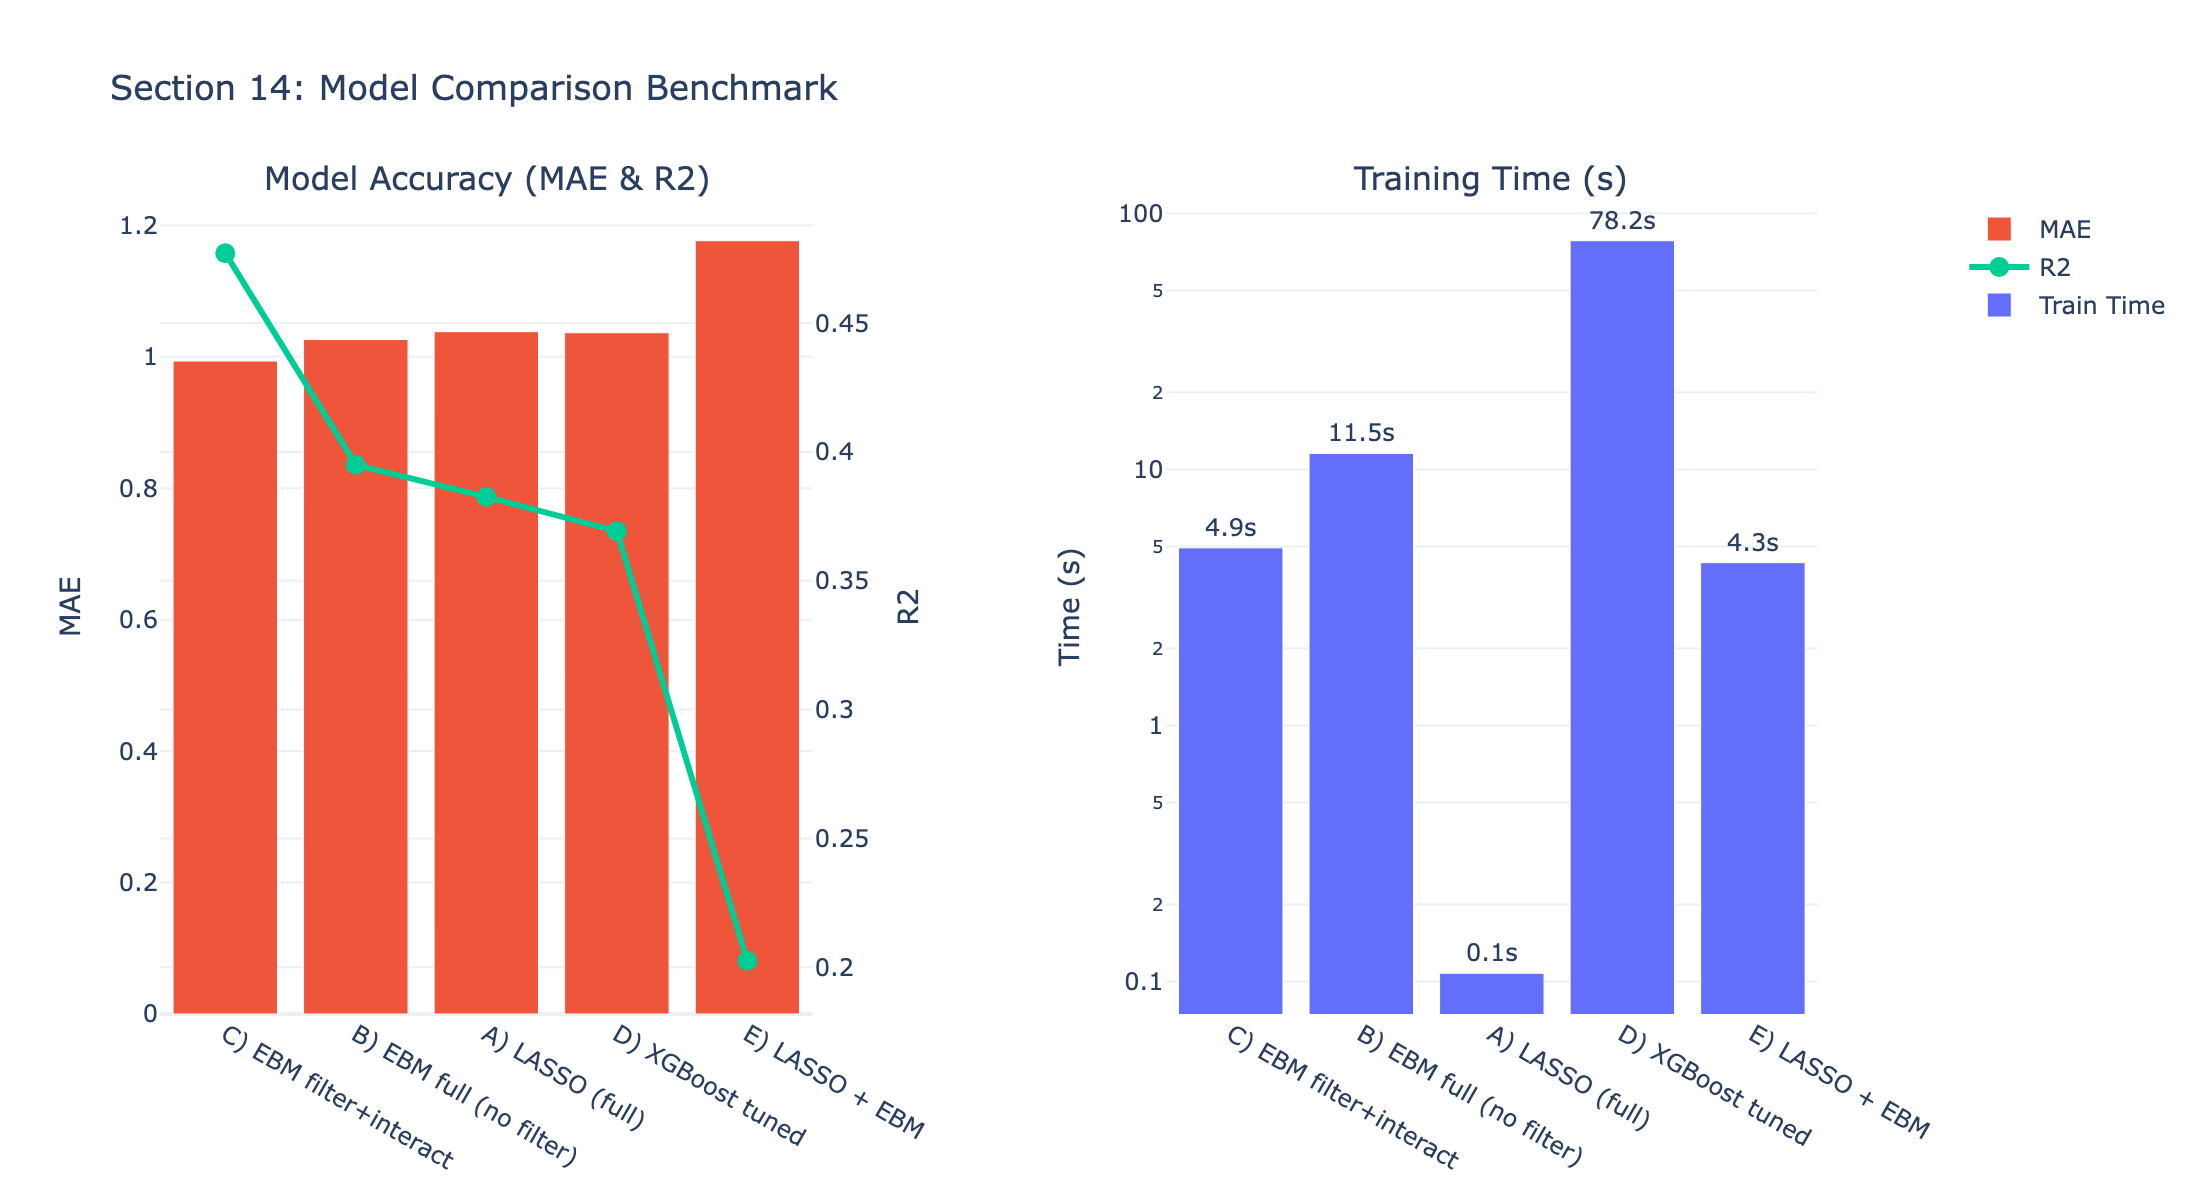
\includegraphics[width=\columnwidth]{images/s14_model_comparison.png}
    \caption{Comparació de rendiment (MAE, R²) i temps d'entrenament dels 5 models avaluats.}
    \label{fig:model_comparison}
\end{figure}

La Figura~\ref{fig:complexity_vs_r2} condensa l'argument central d'aquest treball: el model proposat ocupa la posició òptima a l'espai complexitat-rendiment. Amb només 25 termes interpretables (15 efectes principals + 10 interaccions), supera en R² un XGBoost amb 2.500 paràmetres estimats. Aquesta diferència de dos ordres de magnitud en complexitat té implicacions directes: cada terme del model EBM pot ser revisat, validat i justificat per un enginyer de procés en menys d'una hora, mentre que un XGBoost requereix tècniques post-hoc (SHAP) que afegeixen una capa d'aproximació i incertesa interpretativa \cite{rudin2021fundamental}.

\begin{figure}[htbp]
    \centering
    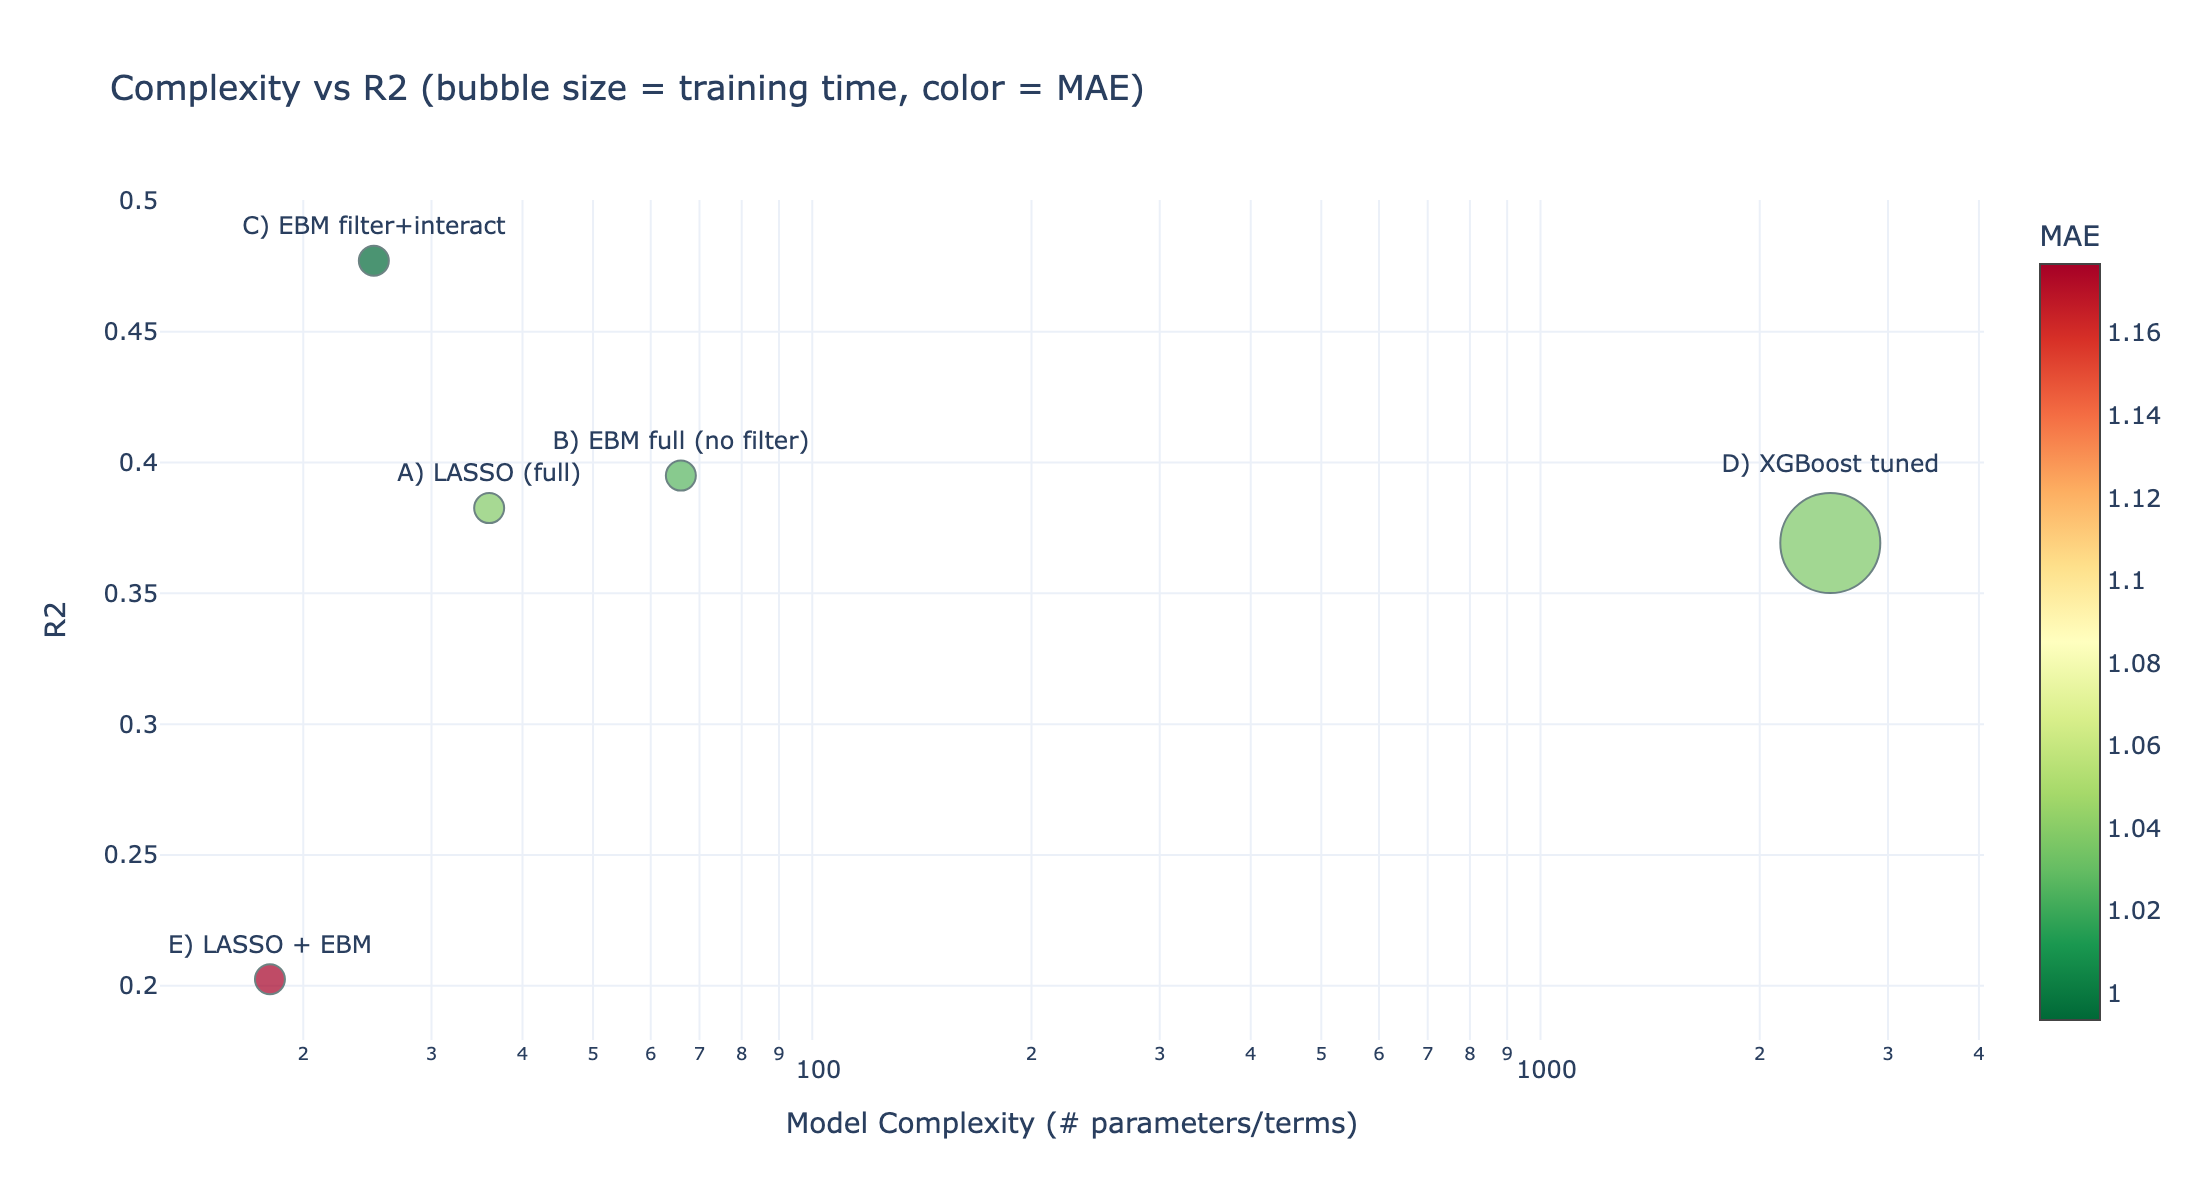
\includegraphics[width=\columnwidth]{images/s14_complexity_vs_r2.png}
    \caption{Compromís complexitat-rendiment: nombre de termes/paràmetres (eix x, escala log) vs R² (eix y). La mida de la bombolla codifica temps d'entrenament i el color, MAE.}
    \label{fig:complexity_vs_r2}
\end{figure}

\subsection{Viabilitat computacional per a industrialització}
\label{subsec:viabilitat_computacional}

La viabilitat d'un sistema RCA en producció no depèn únicament de la precisió predictiva, sinó de la seva capacitat d'operar dins dels requisits temporals del procés. En el context de fraccionament de plasma, on cada lot genera dades finals en un cicle de 24-48h i la presa de decisions ha de ser quasi-immediata per evitar propagació de desviacions, el model ha de complir dos requisits: (1) inferència en temps real per alimentar dashboards operatius, i (2) reentrenament ràpid per adaptar-se a canvis de procés sense aturar el sistema.

\begin{figure}[htbp]
    \centering
    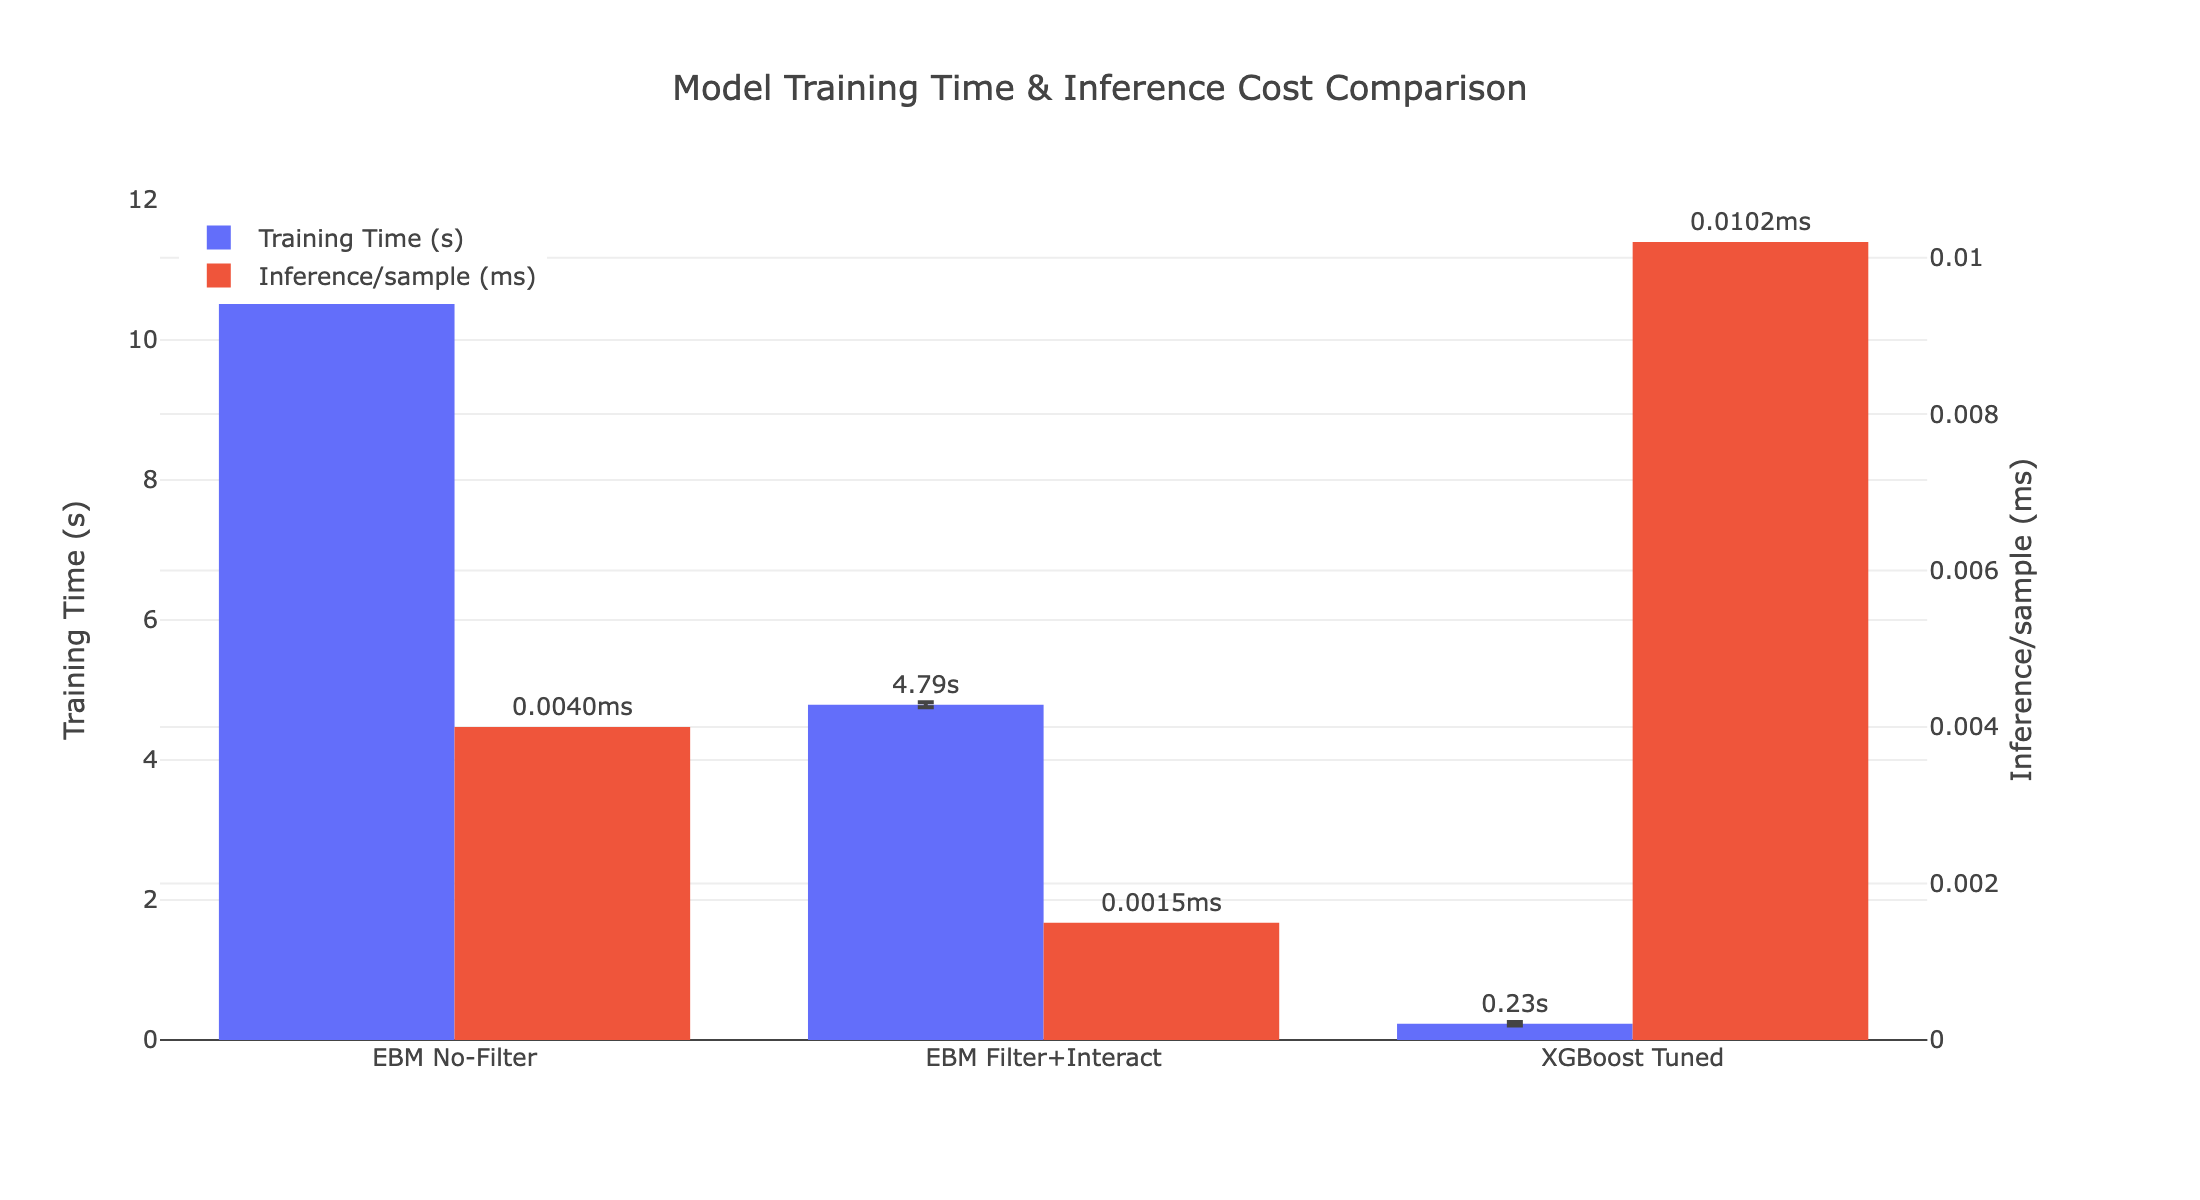
\includegraphics[width=\columnwidth]{images/s15_training_inference_cost.png}
    \caption{Comparació de temps d'entrenament i latència d'inferència entre EBM (amb i sense filtratge) i XGBoost.}
    \label{fig:training_inference_cost}
\end{figure}

La Figura~\ref{fig:training_inference_cost} i la Taula~\ref{tab:computational_viability} demostren que el model proposat compleix ambdós requisits amb marge ampli.

\begin{table}[htbp]
\centering
\caption{Comparació de cost computacional entre models.}
\label{tab:computational_viability}
\scriptsize
\resizebox{\columnwidth}{!}{%
\begin{tabular}{@{}lrrr@{}}
\toprule
\textbf{Mètrica} & \textbf{EBM filter} & \textbf{EBM no-filter} & \textbf{XGBoost} \\
\midrule
Temps entrenament (s) & \textbf{4.8} & 11.4 & 78.2 \\
Latència inferència (ms/mostra) & \textbf{0.0015} & 0.0040 & 0.0102 \\
Throughput (batches/s) & \textbf{688.000} & 248.000 & 99.000 \\
Empremta model (MB) & 2.7 & 4.1 & 0.5 \\
\bottomrule
\end{tabular}%
}
\end{table}

El model proposat aconsegueix la menor latència (0.0015~ms/mostra, equivalent a 688.000 prediccions/segon), permetent processar la totalitat de la producció anual (aprox. 1.000 lots) en menys de 2~ms i la integració directa amb sistemes MES/SCADA sense impacte en els temps de cicle. El temps de reentrenament de 4.8~s habilita una estratègia de reentrenament per lot sense requerir infraestructura de computació dedicada, i l'empremta de 2.7~MB permet desplegament en contenidors lleugers sense GPU, compatible amb arquitectures \emph{edge} en planta.

Des d'una perspectiva de cost operatiu, la combinació de latència mínima i reentrenament ràpid permet desplegar el sistema com a servei continu sense \emph{batch scheduling}, reduint la complexitat d'infraestructura IT i els costos associats de manteniment.

\subsection{Monitoratge retrospectiu de drift}
\label{subsec:monitoratge_drift}

Un model desplegat en producció perd validesa quan les distribucions de les variables d'entrada canvien respecte a les condicions d'entrenament. Per quantificar aquest risc de manera prospectiva, s'ha implementat un sistema de monitoratge basat en el \emph{Population Stability Index} (PSI) sobre finestres lliscants de 50 lots amb pas de 25, avaluant les 5 variables de major importància del model.

La Figura~\ref{fig:drift_psi} mostra els resultats del monitoratge retrospectiu sobre les darreres 290 mostres (30\% del dataset, cronològicament ordenades):

\begin{figure}[htbp]
    \centering
    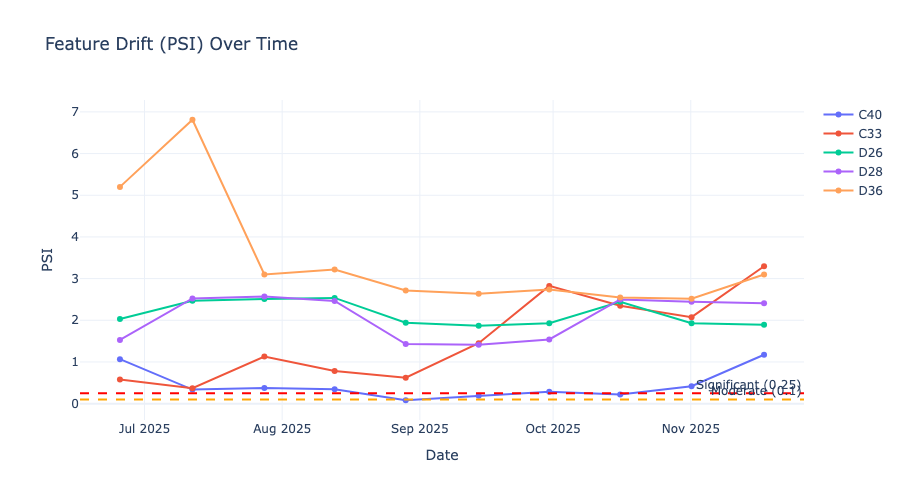
\includegraphics[width=\columnwidth]{images/drift.png}
    \caption{Evolució del PSI per a les 5 variables principals del model. Línia discontínua vermella: llindar de drift significatiu (PSI $>$ 0.25).}
    \label{fig:drift_psi}
\end{figure}

L'anàlisi revela un patró de drift generalitzat des de juny 2025, amb dues observacions críticament rellevants per a la industrialització:

\textbf{(1) Drift extrem en variables de filtració.} D36 (nombre total de papers gruixuts) assoleix PSI=6.8, indicant un canvi radical en la distribució d'aquesta variable — probablement un canvi de material o protocol de filtració. Aquesta magnitud de drift (PSI $>$ 5 és considerat crític en la literatura \cite{lu2020drift}) implica que les shape functions apreses per D36 operen fora del rang d'entrenament, comprometent potencialment la fiabilitat de les contribucions locals.

\textbf{(2) Robustesa del model malgrat el drift.} Malgrat els valors extrems de PSI, el MAE del model sobre les finestres d'avaluació es manté per sota del límit de control superior (UCL=2.55) en totes les finestres. Això demostra que l'estructura additiva de l'EBM proporciona una degradació gradual: quan una variable deriva, les restants 14 variables i 10 interaccions mantenen capacitat predictiva. Tanmateix, la recomanació operativa és activar reentrenament quan qualsevol variable superi PSI $>$ 0.25 durant 3 finestres consecutives, per prevenir acumulació de biaix.

Aquesta anàlisi valida empíricament la necessitat de la capa de monitoratge proposada a la Secció~\ref{subsec:capa_validacio_industrialitzacio} i demostra que el sistema detecta proactivament condicions que requereixen intervenció, abans que es tradueixin en degradació mesurable del rendiment predictiu.

\subsection{Interpretació dels resultats i utilitat per a RCA}

L'anàlisi mostra que el guany predictiu prové de la combinació d'efectes principals i interaccions rellevants, no d'una única variable dominant. Els factors més crítics identificats inclouen variables de condicions de tanc, temps de mescla, configuracions de filtració i estructura operativa del lot. Les interaccions més rellevants combinen variables de preparació i filtració, explicant comportaments no lineals impossibles de captar amb models lineals.

\subsubsection{Avantatge de la interpretabilitat nativa: shape functions vs SHAP}

La Figura~\ref{fig:shape_c33} il·lustra un cas paradigmàtic de la superioritat interpretativa de l'EBM respecte a models \emph{black-box} amb explicabilitat post-hoc. La variable C33 (temps total de mescla de Fracció I) exhibeix una relació fortament no lineal amb el yield D49: el punt òptim se situa a 3.04 minuts (+0.276 punts percentuals de contribució), amb un rang segur entre 1.2 i 9.3 minuts on l'impacte és positiu o neutre. Més enllà de 10 minuts, la penalització creix de manera progressiva fins a $-$0.6~pp per a valors superiors a 35 minuts — un patró de saturació que cap model lineal pot capturar.

\begin{figure}[htbp]
    \centering
    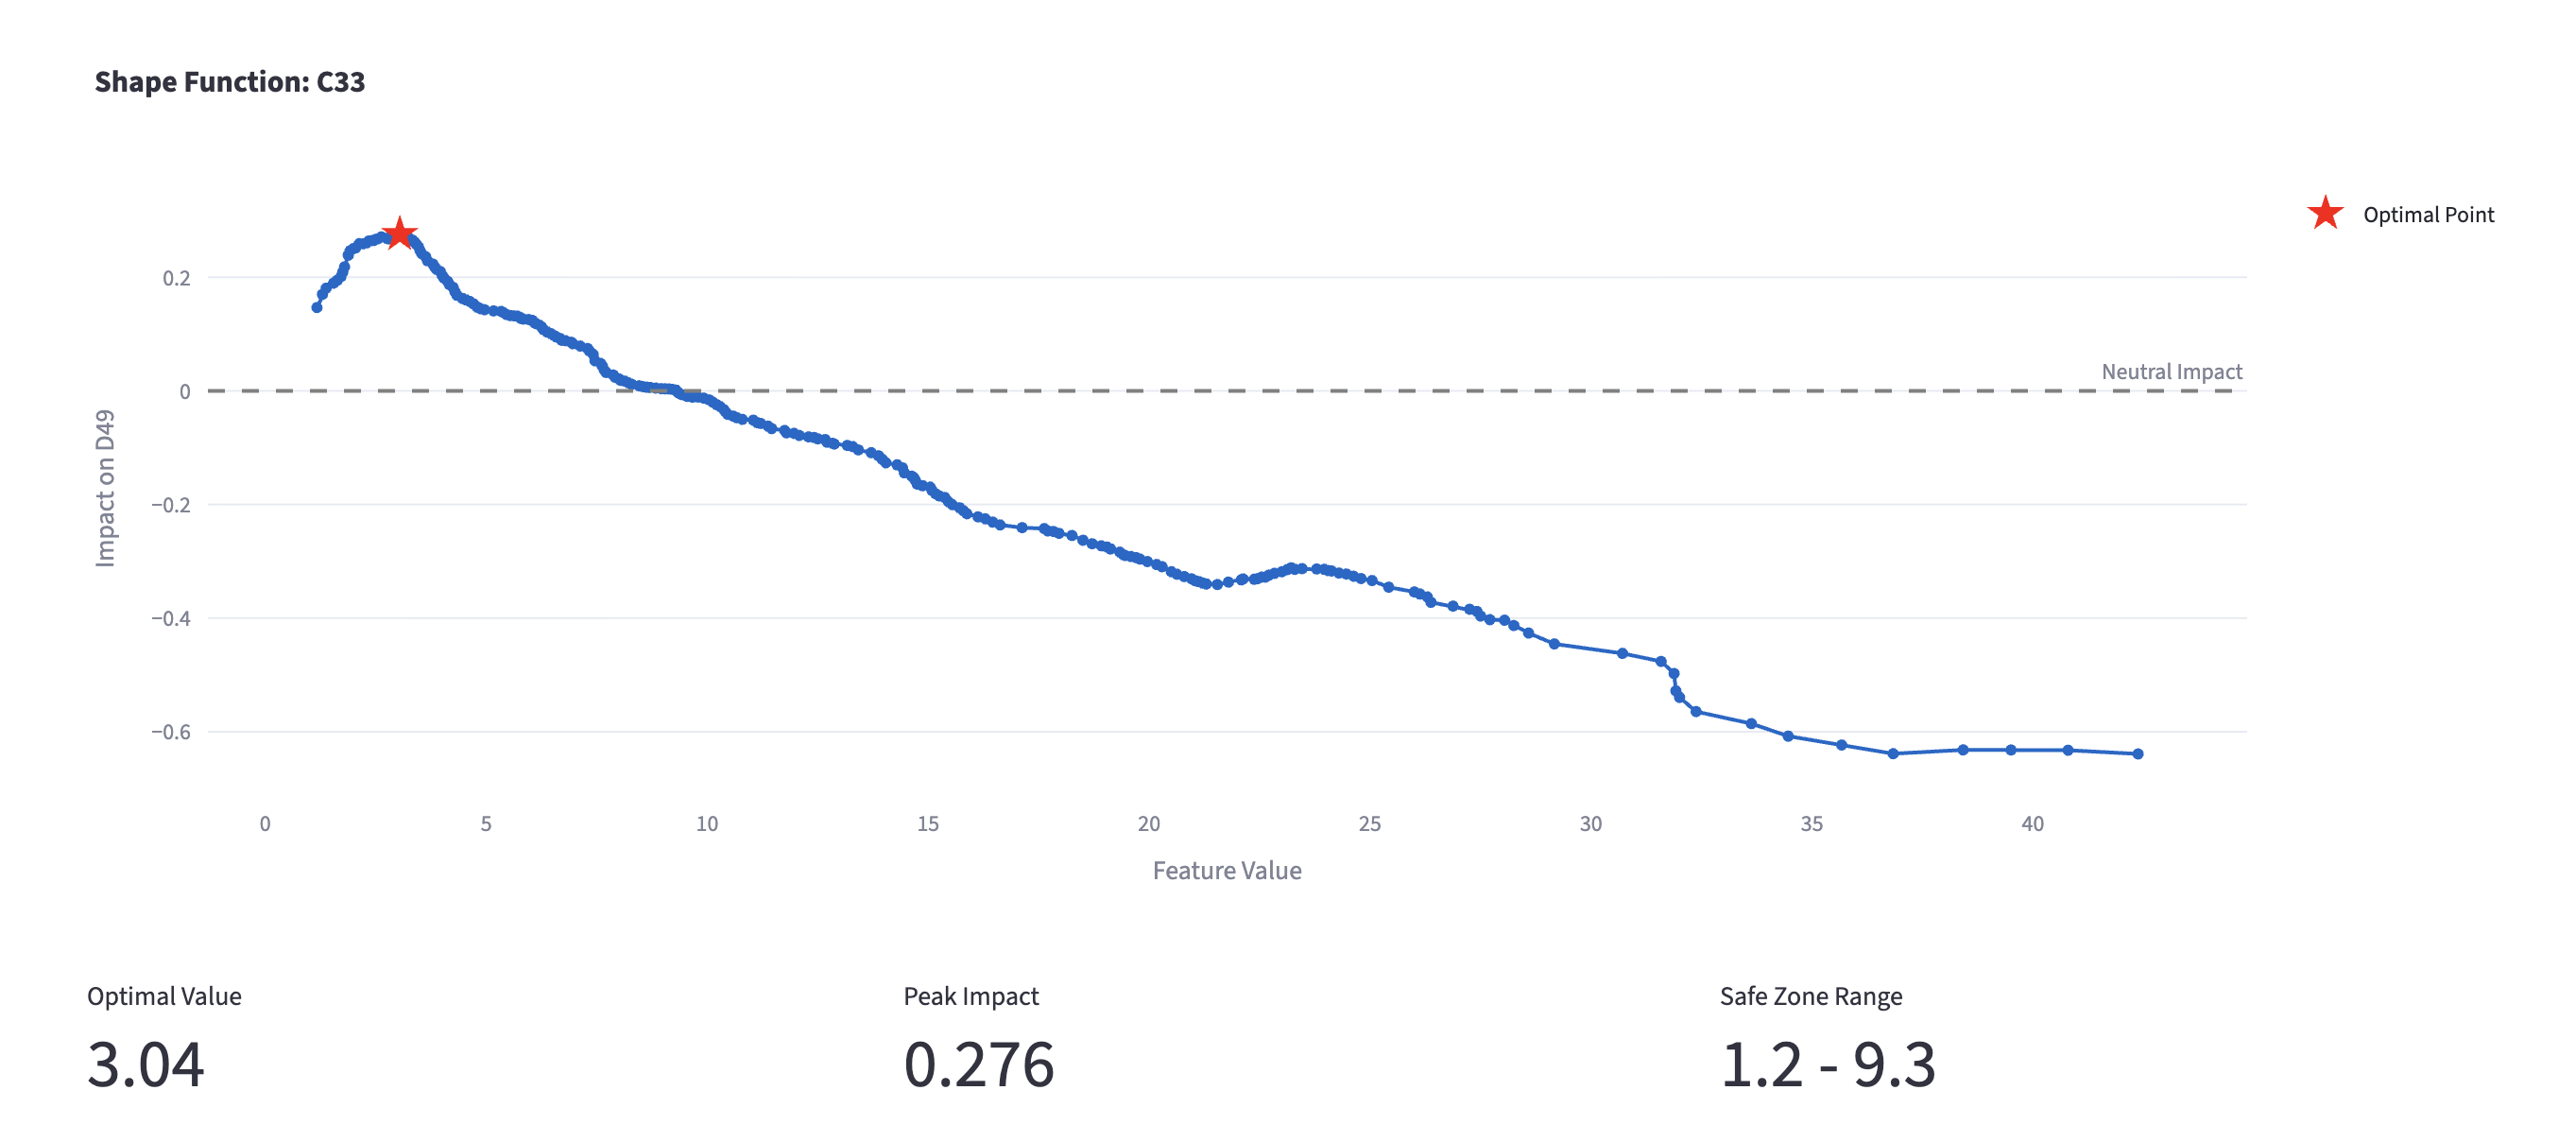
\includegraphics[width=\columnwidth]{images/shape_c33.png}
    \caption{Shape function de C33 (temps total de mescla FI) apresa per l'EBM. La corba mostra la contribució marginal al yield D49: valors propers a 3 minuts maximitzen l'impacte (+0.276 pp), mentre que valors superiors a 10 provoquen penalitzacions creixents fins a $-$0.6 pp. Rang operatiu segur: 1.2--9.3.}
    \label{fig:shape_c33}
\end{figure}

Aquesta informació és directament accionable: un enginyer de procés pot identificar immediatament que el temps de mescla òptim és de 3 minuts, que operar entre 1.2 i 9.3 minuts és segur, i que cada minut addicional per sobre de 10 té un cost quantificable d'aproximadament 0.03~pp de yield — equivalent, al preu de referència de 55~\$/g, a una pèrdua de milers de dòlars per lot. En contrast, l'aproximació \emph{black-box} amb explicabilitat post-hoc (p.~ex. XGBoost + SHAP) presenta tres limitacions fonamentals en aquest context:

\begin{enumerate}
    \item \textbf{Inconsistència entre mètodes post-hoc.} SHAP i LIME poden generar explicacions divergents per a la mateixa predicció, especialment en presència de variables correlacionades \cite{rudin2021fundamental}. L'EBM, en canvi, té una única descomposició exacta per construcció ($f(x) = \beta_0 + \sum_i f_i(x_i) + \sum_{ij} f_{ij}$).

    \item \textbf{Pèrdua d'informació sobre la forma funcional.} SHAP values indiquen la \emph{magnitud} i \emph{direcció} de l'efecte d'una variable per a una observació concreta, però no revelen la \emph{forma} de la relació al llarg de tot el rang. Un enginyer necessita saber no només que ``C33 penalitza en aquest lot'' sinó \emph{per què} (massa curt? massa llarg?) i \emph{quin és el rang òptim}. La shape function de l'EBM respon ambdues preguntes simultàniament.

    \item \textbf{Cost computacional i auditabilitat.} Calcular SHAP values per a un XGBoost amb 2.500 arbres requereix computació significativa per mostra i genera explicacions aproximades. En entorn GxP, on cada explicació ha de ser reproduïble i auditable \cite{gamp5,alcoa}, les aproximacions post-hoc introdueixen un risc de validació addicional que l'EBM evita per disseny.
\end{enumerate}

Des d'una perspectiva operativa, la metodologia redueix l'espai de recerca des del conjunt ampli de variables originals cap a un subconjunt prioritari, facilitant: (1) reducció de complexitat inicial en investigacions RCA; (2) generació d'hipòtesis accionables amb impacte mesurable; (3) traçabilitat de decisions vinculada a evidència quantitativa.

\subsubsection{Impacte operatiu i econòmic del model}

La utilitat de la metodologia proposada rau en la seva capacitat per quantificar el cost d'oportunitat de les desviacions i prioritzar accions de millora basades en evidència quantitativa. Per fonamentar la validesa d'aquestes projeccions, s'ha utilitzat el model configurat com a \textbf{Robust (Leaf=10)}. L'aplicació d'una estratègia de validació creuada de 5 folds suggereix una estabilitat adequada en les mètriques de rendiment (R² = 0.422 i MAE = 0.950 $\pm$ 0.063), redueix el risc de sobreajustament i mostra estabilitat fora de mostra, indicant una capacitat de generalització moderada.

\paragraph{Metodologia d'estimació del potencial optimitzat.} A diferència dels models de caixa negra, l'arquitectura nativament interpretable de l'EBM permet descompondre cada predicció individual com una suma algebraica de contribucions:
\[
f(x) = \beta_0 + \sum_i f_i(x_i) + \sum_{i,j} f_{ij}(x_i,x_j).
\]
Aquesta propietat s'ha utilitzat per identificar, lot a lot, el cost d'oportunitat vinculat a variables operatives subòptimes. El potencial optimitzat de cada lot, $Y_{opt}$, es calcula segons l'expressió següent:
\[
Y_{opt} = Y_{pred} + \left(-Score_{neg} \cdot rec \cdot R^2\right).
\]
On $Score_{neg}$ representa la suma de les contribucions negatives identificades pel model (factors amb impacte inferior a $-0.1$ punts percentuals), i $rec$ és un factor de recuperació operativa fixat en el 70\%. Aquesta penalització del 30\% en la recuperació, sumada a la ponderació per la variància explicada ($R^2=0.422$), constitueix un coeficient de conservadorisme global aproximat del 29.4\%, que integra les limitacions de controlabilitat en planta i les possibles interaccions no lineals no capturades.

Aquest coeficient no és arbitrari, sinó que respon a la integració de dues limitacions fonamentals: (1) \textbf{variància explicada} ($R^2 = 0.422$), que actua com a factor de confiança estadística, assumint que només es pot intervenir sobre la fracció de variabilitat que el model és capaç de capturar; i (2) \textbf{recuperabilitat operativa} ($rec = 0.70$), que aplica una penalització del 30\% per considerar les friccions reals de la planta, com el temps de resposta, la precisió dels equips i les inèrcies del procés. Això reconeix que l'optimització teòrica rarament és assolible al 100\% en entorns GxP. Cal destacar que les contribucions del model s'interpreten com a senyals direccionals associatius, i no com a efectes causals directes sobre el rendiment.

\paragraph{Escenari A: potencial total d'optimització del portfoli.} L'anàlisi de la cartera sobre els lots del període post-canvi revela que la producció presenta oportunitats d'optimització en alguns dels seus paràmetres. En aquest escenari ideal, on es corregirien tots els factors operatius que el model identifica com a \emph{negative drivers}, s'estima un increment del rendiment mitjà (D49) del 46.31\% al 47.32\%. Aquest guany absolut de +1.01 punts percentuals, equivalent a una millora relativa del 2.2\%, suposaria un increment mitjà de facturació de 268.000~\$ per lot produït, assumint un preu de referència de 55~\$/g. En el conjunt del portfoli analitzat, l'oportunitat total ascendeix a 259 milions de dòlars, associats a 4.703 kg de proteïna addicional, amb un impacte recurrent estimat de 26.8 milions de dòlars anuals per a una cadència de 100 lots. Aquest escenari s'ha d'interpretar com un horitzó aspiracional, ja que l'optimització simultània de totes les variables pot veure's limitada per interaccions no lineals o restriccions físiques de la instal·lació.

\paragraph{Escenari B: optimització focalitzada d'alt retorn.} Atès que una intervenció sobre totes les variables pot ser complexa operativament, el model permet identificar una ruta d'optimització simplificada, focalitzada en només tres variables crítiques: D36, paràmetre de filtració que afecta el 62.1\% dels lots; D24, associada a mescla i present en el 50.4\% dels lots; i D40, associada a filtració i present en el 43.0\% dels lots. Aquesta intervenció selectiva permetria capturar de forma immediata un guany de +0.19 punts percentuals de rendiment, aproximadament el 19\% del potencial total del model. Tot i semblar una xifra modesta en termes percentuals, en el context de l'alt valor de la proteïna C activada, aquesta millora focalitzada generaria per si sola uns ingressos addicionals propers als 5 milions de dòlars anuals, justificant la inversió en el sistema de decisió assistida amb un esforç d'ajustament mínim en planta.

\paragraph{Metodologia de càlcul i conservadorisme.} Per garantir la robustesa d'ambdós escenaris davant d'auditories de qualitat, s'ha aplicat un factor de conservadorisme global del 29.4\%. Aquest coeficient no és una agregació lineal de magnituds heterogènies, sinó un filtre en cascada que diferencia la confiança estadística de la viabilitat operativa, seguint principis de prudència en la gestió de riscos en projectes de qualitat biofarmacèutica \cite{rathore2009_qbd}. La confiança del model ($R^2 = 0.422$) actua com a primer tall de prudència, assumint que només és possible intervenir sobre la fracció de variabilitat que el model és capaç d'explicar formalment. La recuperabilitat operativa ($rec=0.70$) aplica una penalització del 30\% per absorbir les inèrcies físiques de la planta i els marges de seguretat GxP, reconeixent que l'òptim teòric és difícilment assolible en la pràctica. Finalment, l'error absolut mitjà (MAE = 0.950) s'utilitza com a referència per filtrar les recomanacions, de manera que el cas de negoci es basi en senyals robustos i no en fluctuacions aleatòries.

Aquesta estructura modular permet justificar que les estimacions no són meres projeccions algorítmiques, sinó un escenari de negoci ajustat a la realitat física i estadística de l'entorn de producció. En aquest sentit, el model actua com un sistema de priorització de decisions operatives basat en evidència, i no com un optimitzador automàtic del procés.

Com a tancament d'aquesta metodologia, i per avaluar la robustesa del cas de negoci davant d'entorns canviants, s'ha analitzat la sensibilitat del projecte davant variacions en les principals hipòtesis econòmiques. Pel que fa al preu base de 55~\$/g, una variació de $\pm$10\% té un impacte proporcional sobre els ingressos estimats, equivalent aproximadament a $\pm$26.800~\$ per lot i $\pm$2.68 milions de dòlars anuals. En tots els casos, el projecte manté una contribució econòmica significativa, indicant una baixa sensibilitat a fluctuacions moderades de mercat. També s'han considerat tres escenaris orientatius d'inversió: un escenari conservador d'aproximadament 1 milió de dòlars anuals, amb retorn altament favorable i immediat; un escenari intermedi d'aproximadament 5 milions de dòlars anuals, en què el cas de negoci continua sent clarament positiu i justificaria per si sol l'estratègia focalitzada de l'Escenari B; i un escenari exigent d'aproximadament 15 milions de dòlars anuals, en què el projecte manté un retorn net positiu, tot i la reducció lògica del marge.

En conjunt, l'anàlisi confirma que el \emph{business case} mostra una robustesa elevada davant les variacions de preu i una sensibilitat moderada al cost d'implementació. Aquest últim és el principal factor de variabilitat en la rendibilitat final, però no compromet la viabilitat financera del projecte.

Un resultat rellevant és que la interpretabilitat s'obté de manera \emph{nativa} amb EBM, no com capa post-hoc. Això implica que les contribucions per variable formen part intrínseca de la predicció, amb descomposició exacta del valor estimat. En comparació amb tècniques post-hoc (SHAP, LIME), l'enfocament natiu redueix inconsistències i simplifica la comunicació amb equips de procés i qualitat \cite{shap_arxiv1705,lime_arxiv1602,rudin2021fundamental}.

\subsection{Comparació amb RCA tradicional i limitacions}

L'enfoc data-driven aporta consistència entre casos, velocitat en priorització i capacitat de tractar múltiples variables simultàniament. Tanmateix, l'RCA tradicional manté fortaleses en profunditat causal contextual i integració de coneixement tàcit. La proposta més robusta és una estratègia \emph{human-in-the-loop}: el model estructura i prioritza l'evidència; l'equip expert valida, contrasta i decideix accions finals. La Figura~\ref{fig:mapa_conceptual} (Apèndix A1) il·lustra esquemàticament ambdós fluxos i el posicionament del sistema ML com a eina de suport dins del procés RCA.

Limitacions identificades: (1) dataset efectiu acotat a 956 mostres; (2) dependència de qualitat de registre; (3) risc de \emph{drift} amb canvis operatius \cite{lu2020drift}; (4) lectura causal limitada per natura observacional; (5) bretxa d'implementació per integració GMP/QMS. El model és un \emph{decision support system}, no substitut de revisió experta.

\section{Conclusions i Treball Futur}

Aquest treball demostra la viabilitat tècnica i operativa d'una metodologia d'industrialització de la Root Cause Analysis basada en models ML interpretables en entorns farmacèutics regulats. La proposta integra preparació de dades, modelització per fases, explicabilitat nativa i criteris de validació en un marc coherent, reproduïble i orientat a decisió.

\textbf{Conclusions principals:}

\begin{itemize}
  \item L'estratègia \emph{filter-then-interact} amb EBM millora consistentment el rendiment respecte al baseline Lasso (reducció 15.6\% MAE, 16.9\% RMSE).
  \item La configuració \textbf{Robust (Leaf=10)} ofereix el millor compromís entre precisió (MAE = 0.950), estabilitat i aplicabilitat industrial, prioritzant robustesa davant R² lleugerament inferior a Fase 3.
  \item La interpretabilitat nativa d'EBM facilita la priorització de causes potencials i accelera la formulació d'hipòtesis RCA, reduint l'espai de recerca i millorant l'eficiència investigadora.
  \item El sistema és especialment útil com a eina de suport en contextos de producció amb alta exigència de traçabilitat, connectant potencial analític del ML amb necessitats operatives de qualitat farmacèutica.
\end{itemize}

Tanmateix, com s'analitza a la Secció~\ref{subsubsec:marc_validacio_gxp}, el treball constitueix el pas previ tècnic necessari abans d'una validació GxP formal (IQ/OQ/PQ): els fonaments —interpretabilitat, traçabilitat i monitoratge— hi són, però la qualificació reguladora i l'aprovació QA resten com a treball futur.

\textbf{Línies de treball futur:}

\begin{itemize}
  \item \textbf{Validació formal GxP:} executar IQ/OQ/PQ i integrar en cicle de validació corporatiu.
  \item \textbf{Ampliació i qualitat de dades:} incrementar cobertura temporal i validar en nous escenaris de producció.
  \item \textbf{Monitoratge i governança:} desplegar seguiment de deriva, versionat, protocols de recalibratge i reentrenament amb aprovacions QA.
  \item \textbf{Integració operativa:} connectar priorització RCA amb fluxos de desviacions, CAPA i sistemes MES/LIMS.
\end{itemize}

Com a conclusió final, la proposta constitueix una base sòlida, escalable i auditable per a la implantació progressiva d'un sistema RCA assistit per ML en entorns regulats, confirmant que és possible evolucionar des d'un RCA qualitatiu cap a un enfoc híbrid, sistemàtic i data-driven, mantenint l'expertesa humana com a element central de validació i decisió final.


\section*{Ús de la Intel·ligència Artificial}

En el desenvolupament d'aquest treball s'han utilitzat tres eines d'IA generativa com a suport:

\begin{itemize}
    \item \textbf{Claude (Anthropic):} Assistència en programació (depuració de codi Python, optimització de pipelines de dades, generació d'scripts per a visualització i benchmarking), revisió i redacció (estructuració de seccions, correcció d'estil i formatació LaTeX), i anàlisi exploratòria (discussió de resultats, interpretació de shape functions i formulació d'hipòtesis).
    \item \textbf{Perplexity AI:} Recerca bibliogràfica i exploració de l'estat de l'art — cerca de publicacions rellevants sobre EBM, GAMs, drift monitoring i validació en entorns GxP, així com verificació de cites i fonts.
    \item \textbf{Gemini (Google):} Suport complementari en revisió de textos, generació de resums i contrast d'idees durant les fases inicials del projecte.
\end{itemize}

En tots els casos, l'autor ha mantingut el criteri de decisió, la validació dels resultats i la responsabilitat sobre el contingut final. La IA no ha participat en la presa de decisions metodològiques ni en la interpretació de domini del procés farmacèutic.

\section*{Agraïments}

Vull agrair al meu tutor Joan Piedrafita el suport i orientació durant tot el projecte.

\renewcommand{\refname}{Bibliografia}
\bibliographystyle{plain}
\bibliography{references}

\onecolumn
\section*{Apèndix}

\subsection*{A1. Planificació temporal del projecte}

% TODO: Inserir diagrama de Gantt
\begin{center}
\textit{[Diagrama de Gantt -- pendent d'inserir]}
\end{center}

\subsection*{A2. Diagrama del procés RCA}

\begin{figure}[H]
    \centering
    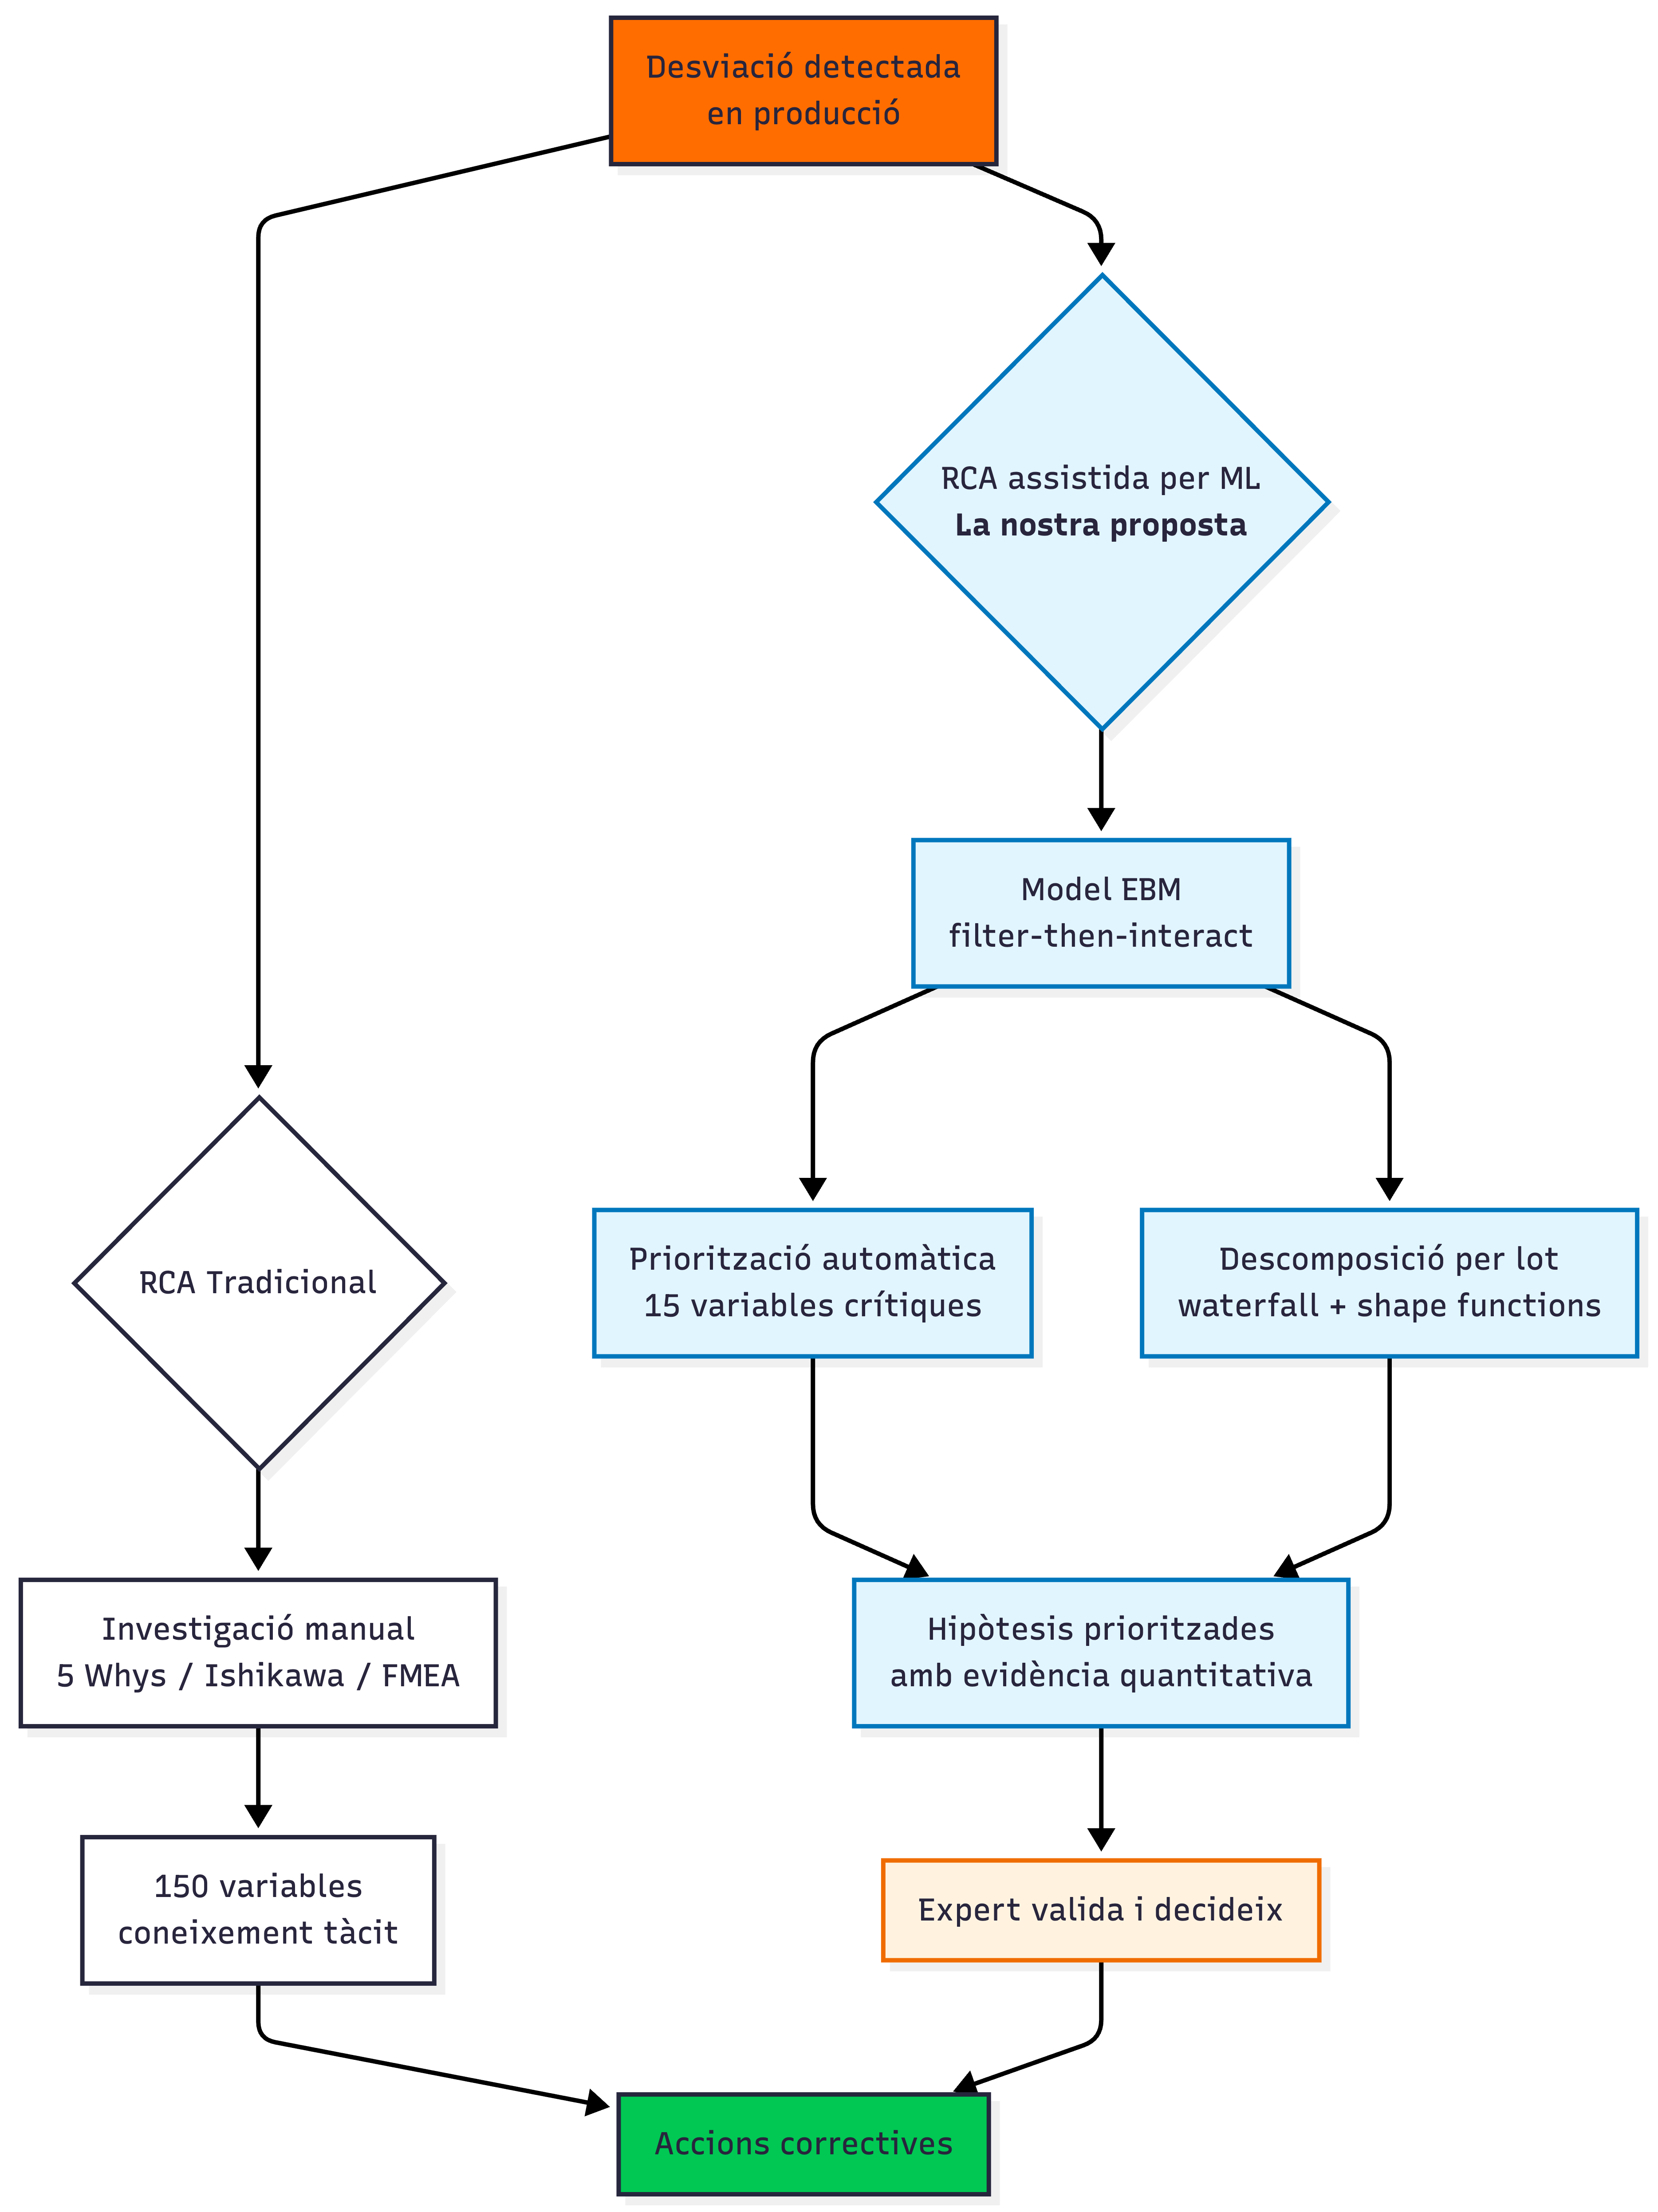
\includegraphics[width=0.85\textwidth]{images/mapa-conceptual.png}
    \caption{Comparació del flux RCA tradicional (manual) i el flux RCA assistit per ML proposat en aquest treball. El sistema ML prioritza hipòtesis amb evidència quantitativa; l'expert manté el control de la decisió final (\emph{human-in-the-loop}).}
    \label{fig:mapa_conceptual}
\end{figure}

\end{document}
